\chapter{Conclusioni}\label{ch:conclusioni}

\section{Risultati degli esperimenti sui toy-dataset}

\subsection{Parametro k e dimensione del dataset}
\label{sec:res-k-dataset-dim}

I primi esperimenti che abbiamo proposto nel capitolo precedente \ref{sec:toy-dataset} erano quelli relativi al robustezza delle metriche alla variazione degli iperparamentri quali \texttt{k} e la dimensione del dataset \(|\Phi|\).
In particolare ci siamo posti come obiettivo di riprodurre le heatmap presenti in \cite{3ReliableFidelityDiversityMetrics} per il confronto delle metriche di precisione-recall e density-coverage con distribuzioni normali per i dataset, ed estenderli a distribuzioni uniformi e alle metriche non analizzate dal paper.

\begin{figure}[!ht]
    \centering
    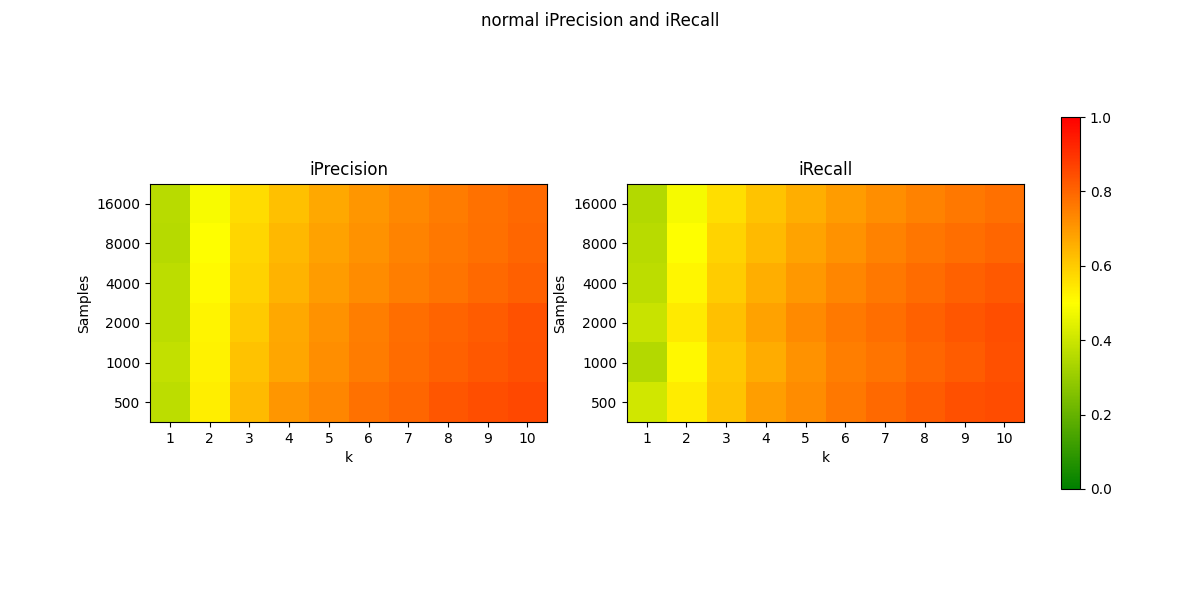
\includegraphics[width=0.8\textwidth]{../images/toyexperiments/kdim/normal_iPrecision_iRecall.png} 
\end{figure}

\begin{figure}[!ht]
    \label{fig:toyexperiments-kdim-normal}
    \centering
    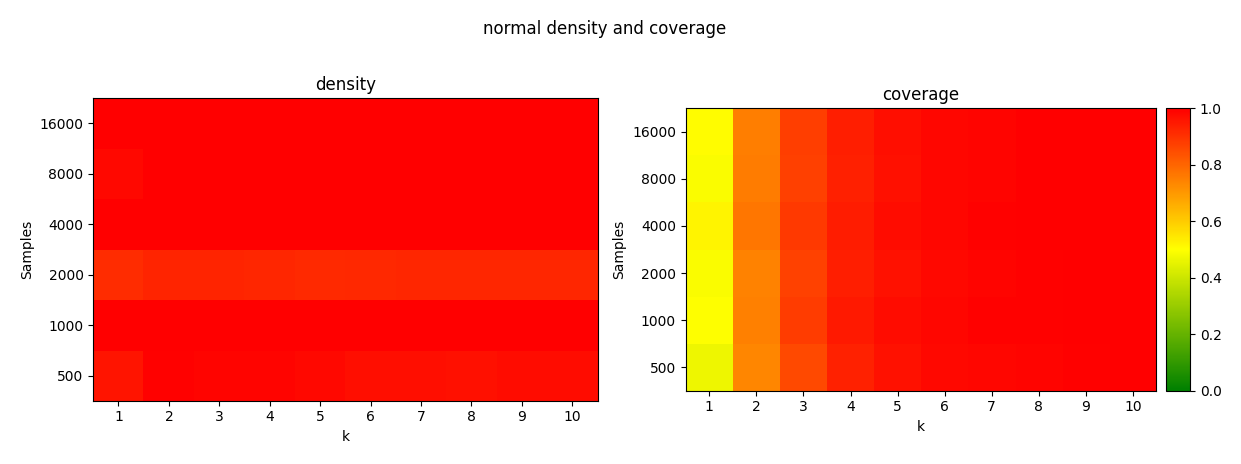
\includegraphics[width=0.8\textwidth]{../images/toyexperiments/kdim/normal_density_coverage.png} 
    \caption{Riproduzione delle heatmap presenti in Reliable Fidelity and Diversity Metrics for Generative Models \cite{3ReliableFidelityDiversityMetrics} per distribuzioni normali di dati}
\end{figure}

Come possiamo notare dai risultati in figura \ref{fig:toyexperiments-kdim-normal}, i risultati ottenuti sono molto simili a quelli presenti nel paper. Essendo le due distribuzioni di dati reali e generati identiche, una metrica che rispecchi tale somiglianza dovrebbe avere valori molto vicini ad \texttt{1.}, in particolar modo quando la dimensione del dataset è molto grande.
Un comportamento simile indicherebbe una buona robustezza della metrica rispetto a variazioni di \texttt{k}, ma come possiamo notare dai grafici, l'improved precision recall è molto più sensibile rispetto ai valori dell'iperparametro. 
Si può notare inoltre una sensibilità maggiore delle metriche al variare di \texttt{k} rispetto alla dimensione del dataset, i grafici sono infatti caratterrizati da colonne verticali di valori/colori molto simili.
La density dall'altra parte è molto più stabile, è però necessario ricordare che per distribuzioni di dati molto simili, non essendo normalizzata, ottenga valori persino maggiori di \texttt{1.}, portando la metrica a non essere molto significativa.
La coverage risulta anch'essa molto stabile, non dando valori molto diversi da \texttt{1.}, ad eccezione per \texttt{k = 1} con dimesione del dataset molto piccola.

C'è poi un altro elemento degno di nota che delude le aspettative ma che è perfettamente logico se si considera la natura delle metriche: l'improved precision-recall ottiene valori maggiori per dimensioni del dataset minori. Il motivo è che la metrica è basata sulla distanza fra i \texttt{k}-NN, e per dataset di dimensione ridotta, la distanza fra i \texttt{k}-NN è maggiore, portando a sovrastimare l'area del manifold di \(R\). Infatti il manifold ricopre un area che cresce quadraticamente rispetto alla distanza fra i campioni, e quando questi si fanno più radi il manifold cresce più velocemente andando ad includere più campioni (nonostante questi siano come detto più distanti fra loro).

Si riportano quindi i risultati per le due metriche ignorate dal paper sempre per distribuzioni normali di dati:

\begin{figure}[!ht]
    \centering
    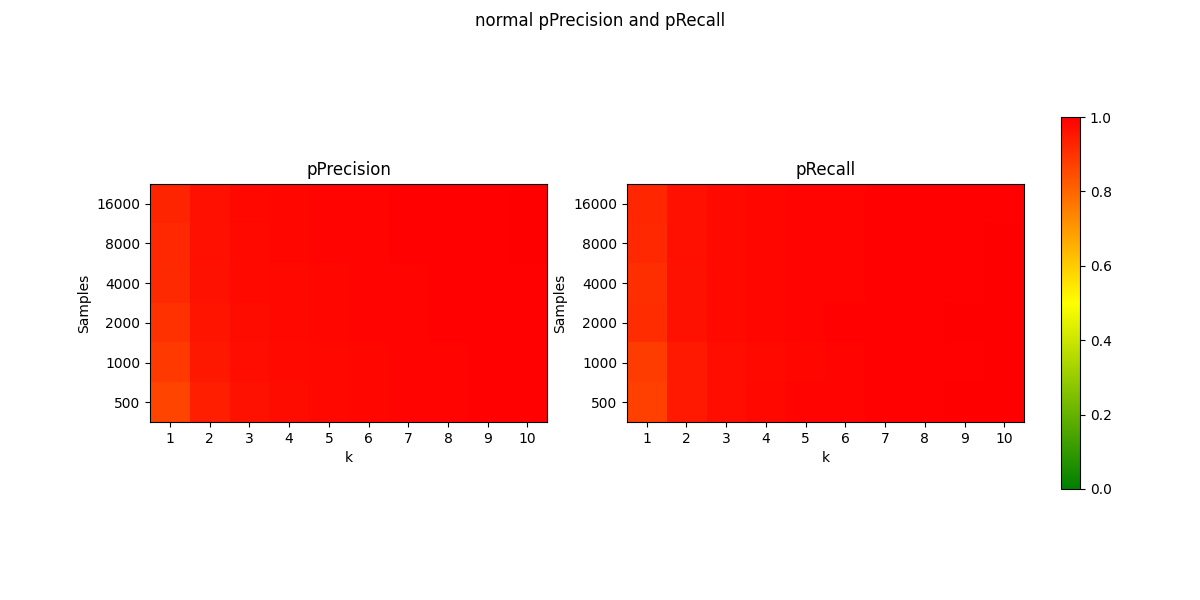
\includegraphics[width=0.8\textwidth]{../images/toyexperiments/kdim/normal_pPrecision_pRecall.png} 
    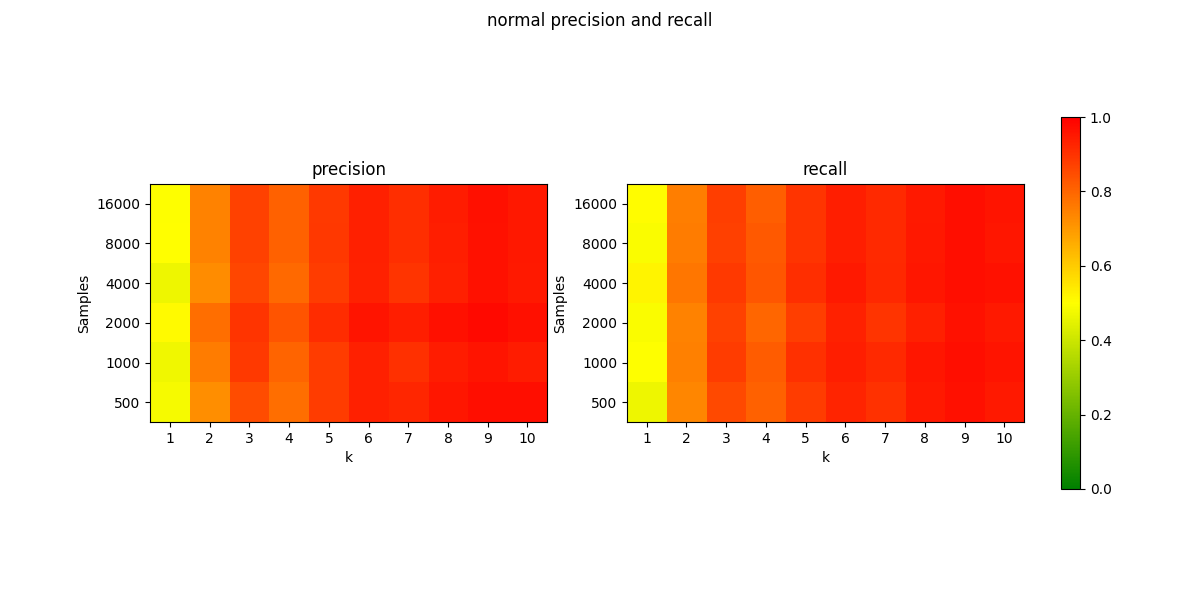
\includegraphics[width=0.8\textwidth]{../images/toyexperiments/kdim/normal_precision_recall.png} 
    \caption{Risultati per la probabibilistic precision-recall e la precision-recall coverage per distribuzioni normali di dati}
\end{figure}

In questo caso è apprezzabile l'uniformità di colore nei grafici della probabibilistic precision e recall, indice della corretta stima della sovrapposizione dei supporti dei dataset di eguale distribuzione.
Come per la density però, dobbiamo limitare i ragionamenti induttivi delle capacità della metrica di stimare la somiglianza fra due distribuzioni, a distribuzioni uguali. Questo vuol dire che con distribuzioni diverse la metrica potrebbe non risultare altrettanto sensibile e appunto continuare a dare valori alti quando non dovrebbe. 
Per la precision-recall coverage invece è interessante notare come per il valore di \texttt{k} consigliato in letteratura (\texttt{k = 3}) questa porti a una stima migliore persino che nel caso di \texttt{k} di valore superiore, dove teoricamente (esclusivamente per distribuzioni identiche), ci si aspetta stime migliori. 
Inoltre si può apprezzare la somiglianza fra i grafici della coverage e della precision-coverage, per i quali ricordiamo dalla teoria che con \texttt{k = 1} le due metriche risultano analiticamente identiche.

I risultati degli esperimenti su distribuzioni uniformi identiche sono i seguenti:

\begin{figure}[!ht]
    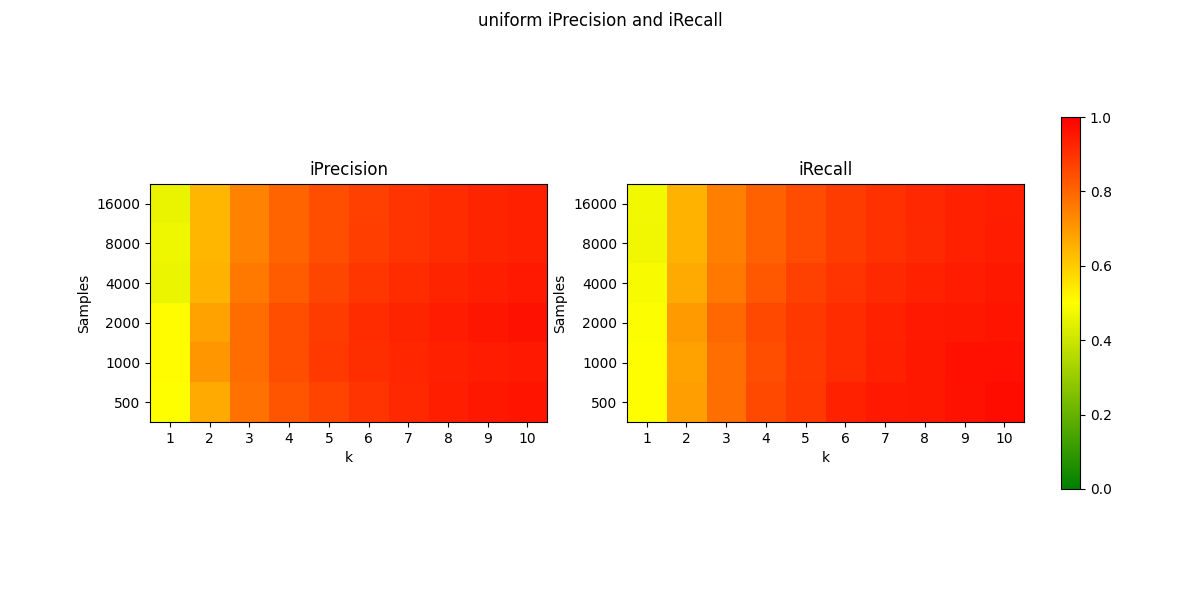
\includegraphics[width=0.5\textwidth]{../images/toyexperiments/kdim/uniform_iPrecision_iRecall.png} 
    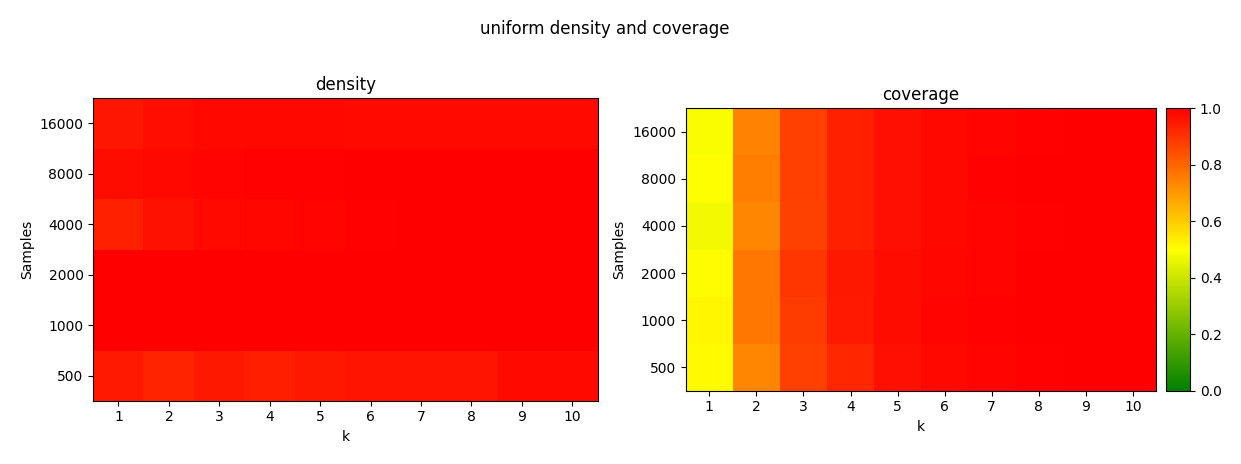
\includegraphics[width=0.5\textwidth]{../images/toyexperiments/kdim/uniform_density_coverage.png} 
    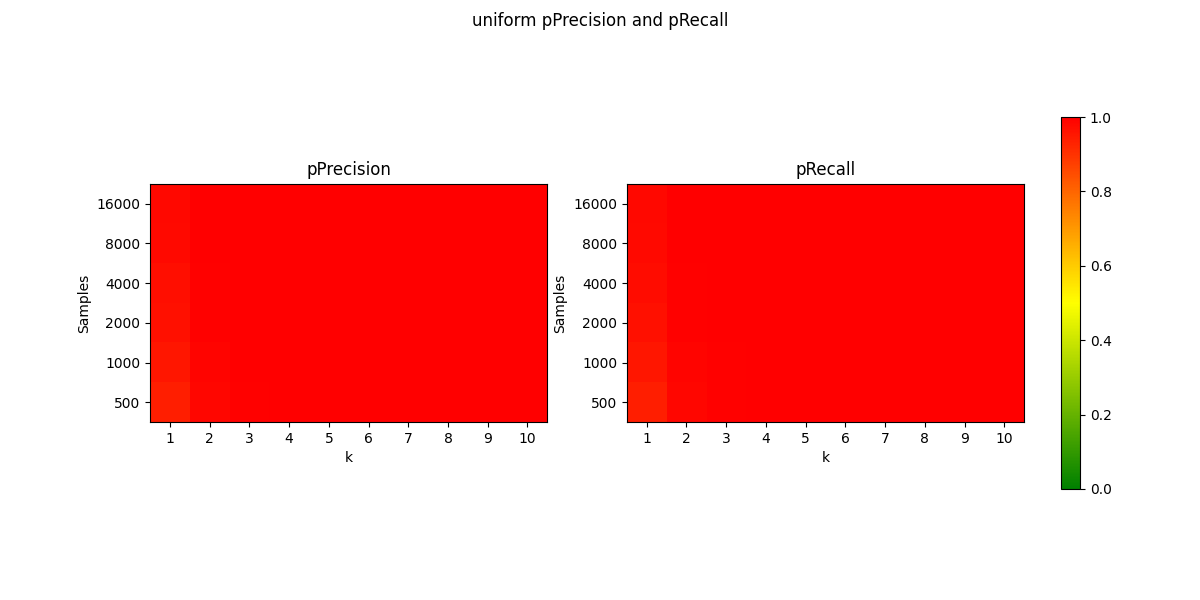
\includegraphics[width=0.5\textwidth]{../images/toyexperiments/kdim/uniform_pPrecision_pRecall.png}
    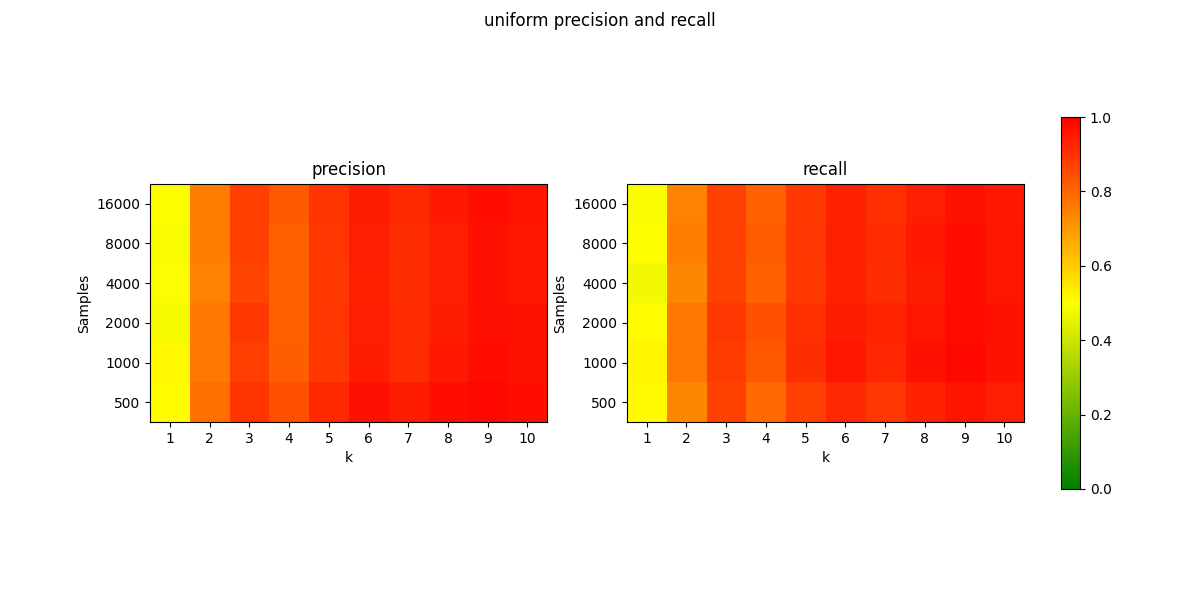
\includegraphics[width=0.5\textwidth]{../images/toyexperiments/kdim/uniform_precision_recall.png}
    \caption{Risultati per distribuzioni uniformi di dati identiche} 
\end{figure}

Come risulta a prima vista, non si discostano molto da i grafici ottenuti con distribuzioni normali. Possiamo quindi solo estendere le precedenti conclusioni a questa nuova distribuzione.
Unica eccezione è l'improved precision-recall che presenta risultati migliori in questo caso, segnalando una limitatezza della sensibilità in presenza di \texttt{k} con valori bassi e distribuzioni normali.

\subsection{Dimensione del dataset e dimensione dei dati}
\label{sec:res-dataset-data-dim}

Per quanto riguarda gli esperimenti sulla dimensione dei dati i risultati sono i seguenti:

\begin{figure}[!ht]
    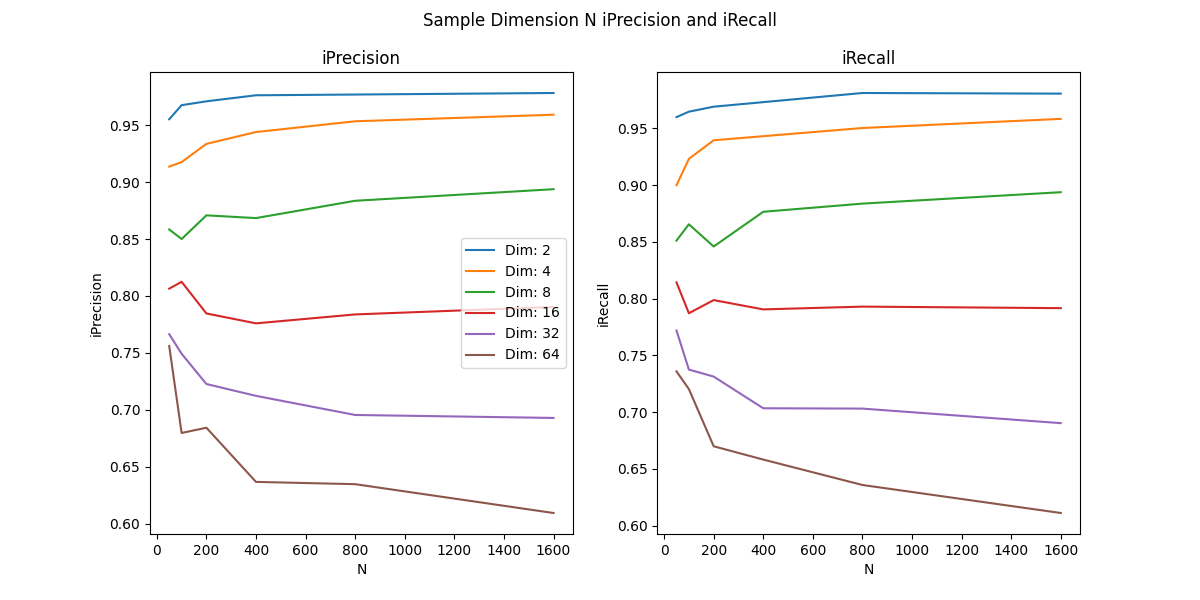
\includegraphics[width=0.5\textwidth]{../images/toyexperiments/ksampledim/sampleDimN_iPrecision_iRecall.png} 
    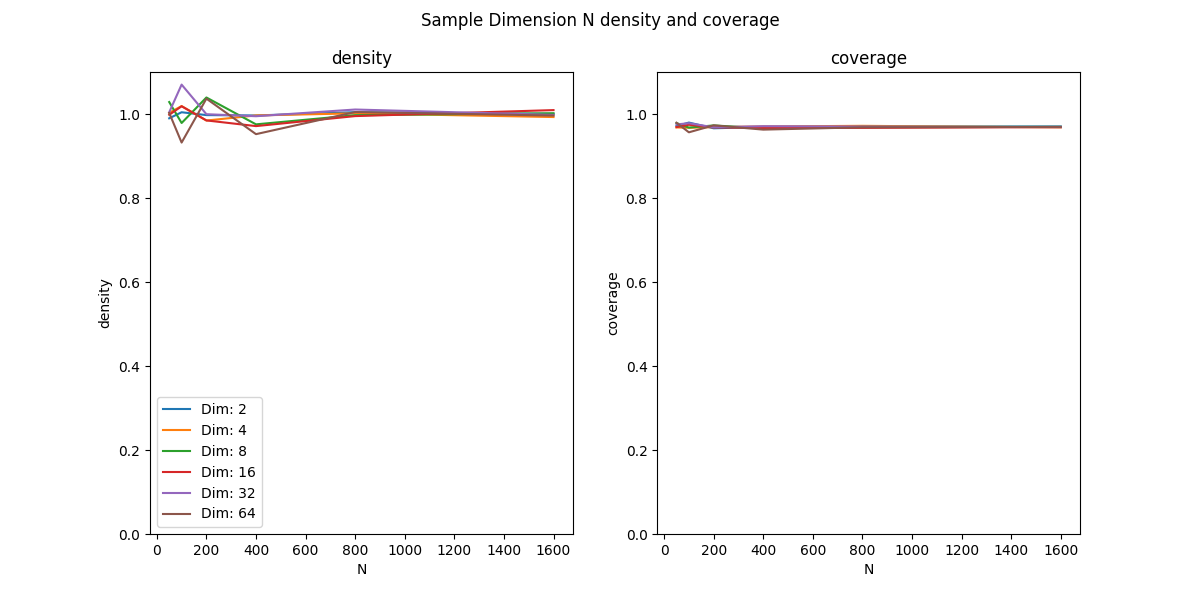
\includegraphics[width=0.5\textwidth]{../images/toyexperiments/ksampledim/sampleDimN_density_coverage.png} 
    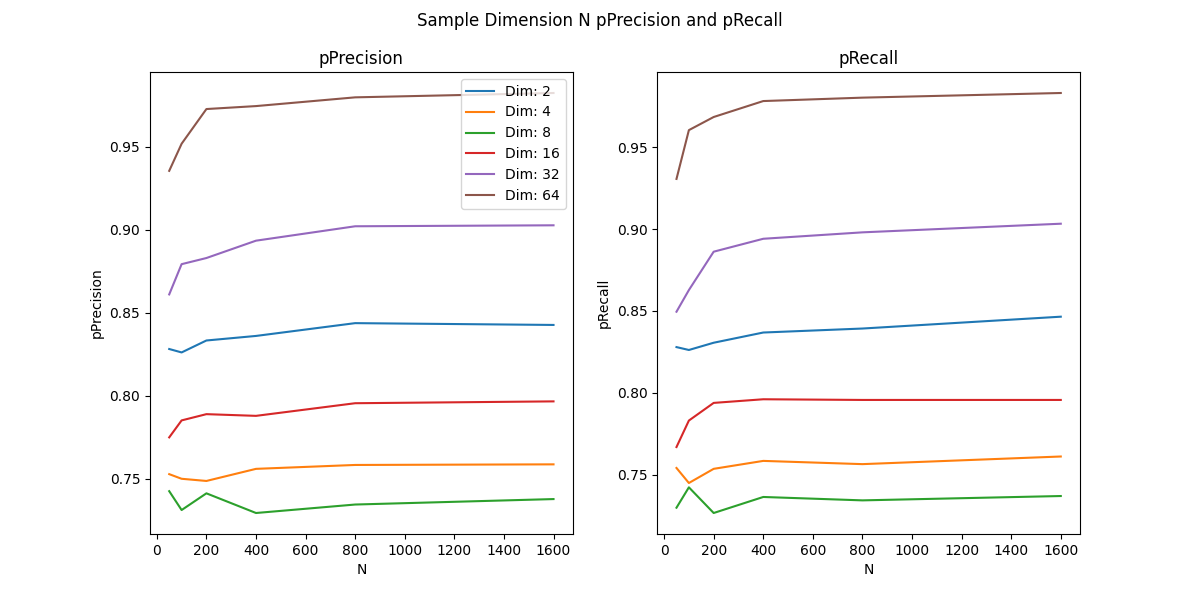
\includegraphics[width=0.5\textwidth]{../images/toyexperiments/ksampledim/sampleDimN_pPrecision_pRecall.png} 
    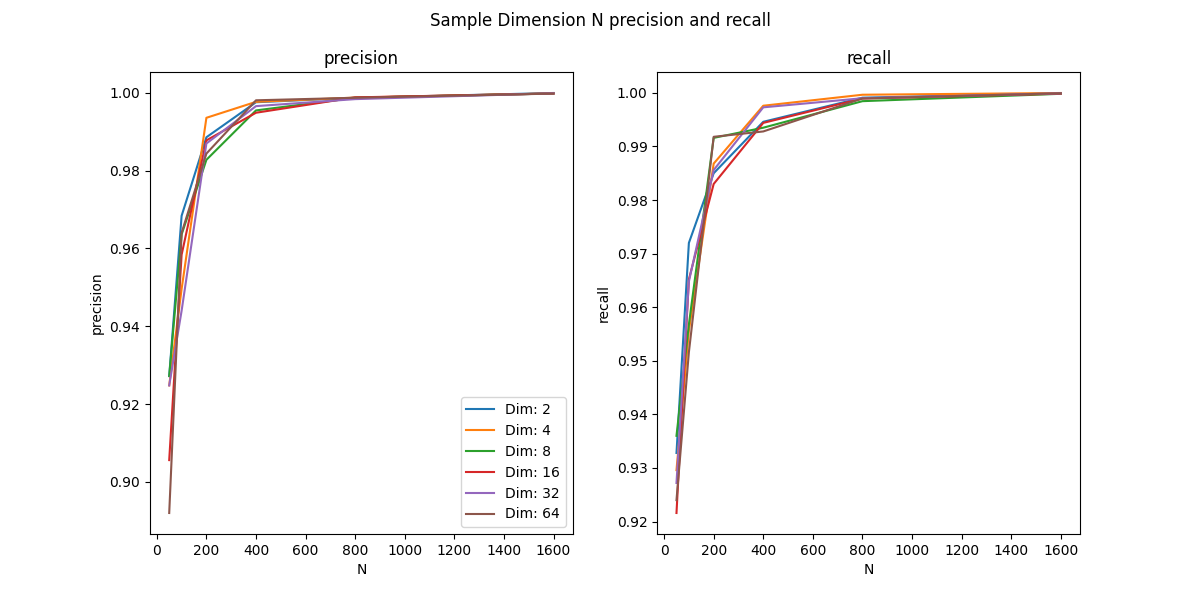
\includegraphics[width=0.5\textwidth]{../images/toyexperiments/ksampledim/sampleDimN_precision_recall.png} 
    \caption{Risultati per la variazione della dimensione dei dati, da sinistra a destra e dall'alto in basso le metriche sono: improved precision-recall, density-coverage, probabilistic precision-recall, precision-recall coverage}
\end{figure}

Le uniche due metriche che risultano sensibili alla variazione della dimensione dei dati sono la improved precision-recall e la probabibilistic precision-recall, mentre le altre due risultano molto stabili.
L'asse delle ascisse è stata limitata leggermente sopra a \texttt{1.} (\texttt{1.25}) possiamo quindi apprezzare visimamente una delle proprietà di cui abbiamo accennato nella sezione precedente e nel primo capitolo:
la density non essendo normalizzata presenta valori che superano il limite logico delle condiviso dalle altre metriche.

Per l'improved precision recall si individua la fragilità della metrica alla dimensione dei dati. Per dimensioni elevate, a parità di numero di campioni e di distribuzione, si registra valori di precision e recall inferiori.
Risulta infatti che per dati in \(\mathbb{R}^{64}\) i valori della metrica siano inferiori di circa 30 punti percentuale rispetto a i dati in  \(\mathbb{R}^{2}\). Si nota inoltre lo stesso difetto visto nella sezione precedente \ref{sec:res-k-dataset-dim}, ovvero che la metrica risulta produrre valori migliori per dimensioni dei dati minori.
Le ragioni sono le stesse, la distanza interna fra i dati è maggiore e quindi il manifold viene sovrastimato.

Per la probabilistic precision recall è sempre presente questa fragilità, ma non è ben chiaro come la dimensione dei dati sia legata agli effettivi risultati della metrica, risulta infatti che per le due dimensioni dei dati maggiori
testate i valori della metrica siano migliori ma con essi è presente anche la dimensione dei dati minore testata, mentre per \(\mathbb{R}^{8}\) otteniamo la stima più bassa.

\subsection{Outliers}
\label{sec:res-outliers}

I casi di studio, come detto nel capitolo precedente sono tre: valori della metrica per distribuzioni normali di dati reali e generate, con la distribuzione dei dati generati centrata nei diversi valori dell'ordinata senza outliers, con outliers nei dati reali e con outliers nei dati generati.

I risultati ottenuti per l'improved precision-recall sono riportati nell immagine \ref{fig:toyexperiments-outliers}. 

\begin{figure}[!ht]
    \label{fig:toyexperiments-outliers}
    \centering
    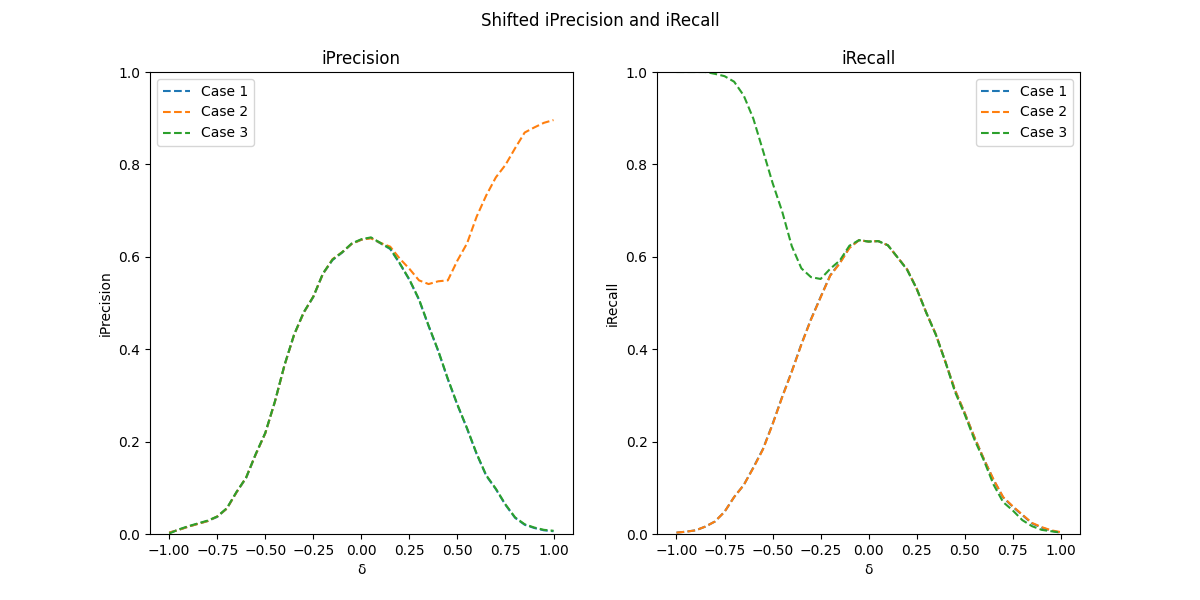
\includegraphics[width=0.8\textwidth]{../images/toyexperiments/outliers/shift_iPrecision_iRecall.png} 
    \caption{Risultati per la resistenza della improved precision-recall alla presenza di outliers nei dati, riprodotto da Reliable Fidelity and Diversity Metrics for Generative Models \cite{3ReliableFidelityDiversityMetrics}}
\end{figure}

È possibile notare che i risultati ottenuti rispettano quanto atteso dalla letteratura. La metrica risulta essere molto sensibile alla presenza di outliers nei dati.
In particolare la precision risulta essere estremamente sensibile alla presenza di outliers nei dati \textbf{reali}, poichè questi vanno a determinare una sovrastimare dell'area del manifold di \(R\), dall'altra parte 
la recall risulta essere molto sensibile alla presenza di outliers nei dati \textbf{generati}, poichè in questo caso si va a sovrastimare l'area del manifold di \(G\).
Un singolo dato outlier può far variare la metrica dell'80\% rispetto al caso senza outliers.
Un altro problema grave delle due metriche è che quando lo shift fra le due distribuzioni è \texttt{0.} la metrica è molto più bassa di \texttt{1.}, paradossalmente viene registrato un valore maggiore dei manifold per distribuzioni con media spostata rispetto a distribuzioni con media centrata.

I risultati ottenuti per la density-coverage sono i seguenti:

\begin{figure}[!ht]
    \centering
    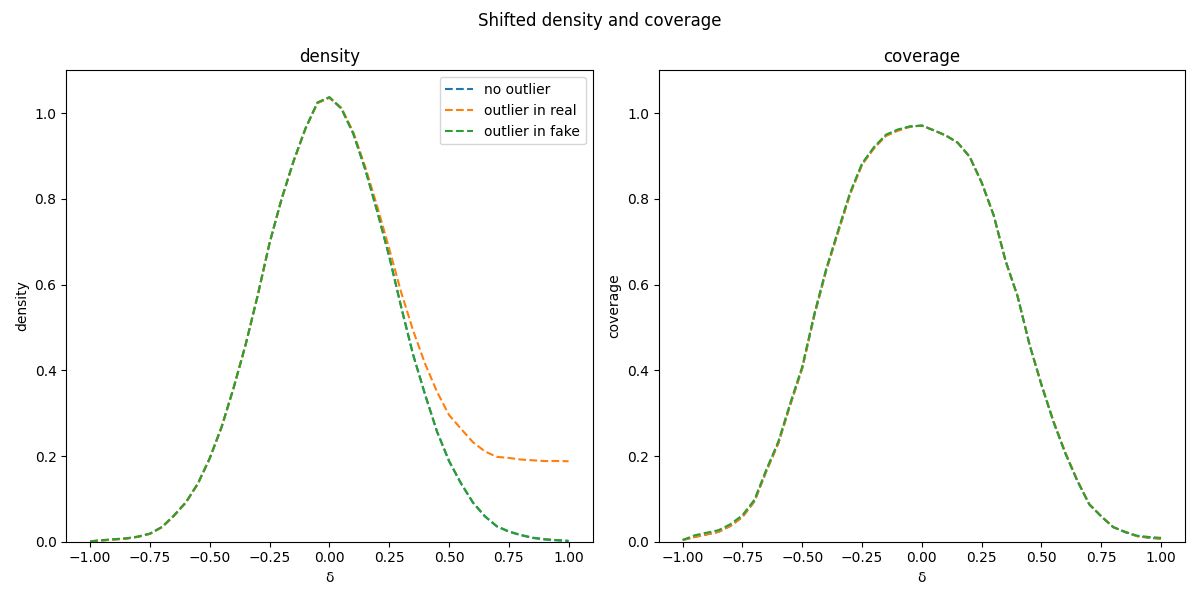
\includegraphics[width=0.8\textwidth]{../images/toyexperiments/outliers/shift_density_coverage.png} 
    \caption{Risultati per la resistenza della density-coverage alla presenza di outliers nei dati, riprodotto da Reliable Fidelity and Diversity Metrics for Generative Models \cite{3ReliableFidelityDiversityMetrics}}
\end{figure}

Ancora una volta i risultati ottenuti rispettano quanto atteso dalla letteratura. La metrica risulta essere molto robusta alla presenza di outliers nei dati.
La density è leggermente influenzata dalla presenza di outliers nei dati reali, ma non in maniera significativa, mentre la coverage non risente della presenza di outliers sia nei dati reali che nei dati generati.
Al contrario dell'improved precision recall, la density e la coverage hanno valori molto vicini a \texttt{1.} quando lo shift fra le due distribuzioni è \texttt{0.} (la density non essendo normalizzata ha valori maggiori di \texttt{1.}).

Per le altre due metriche non indagate nel paper i risultati sono i seguenti:

\begin{figure}[!ht]
    \centering
    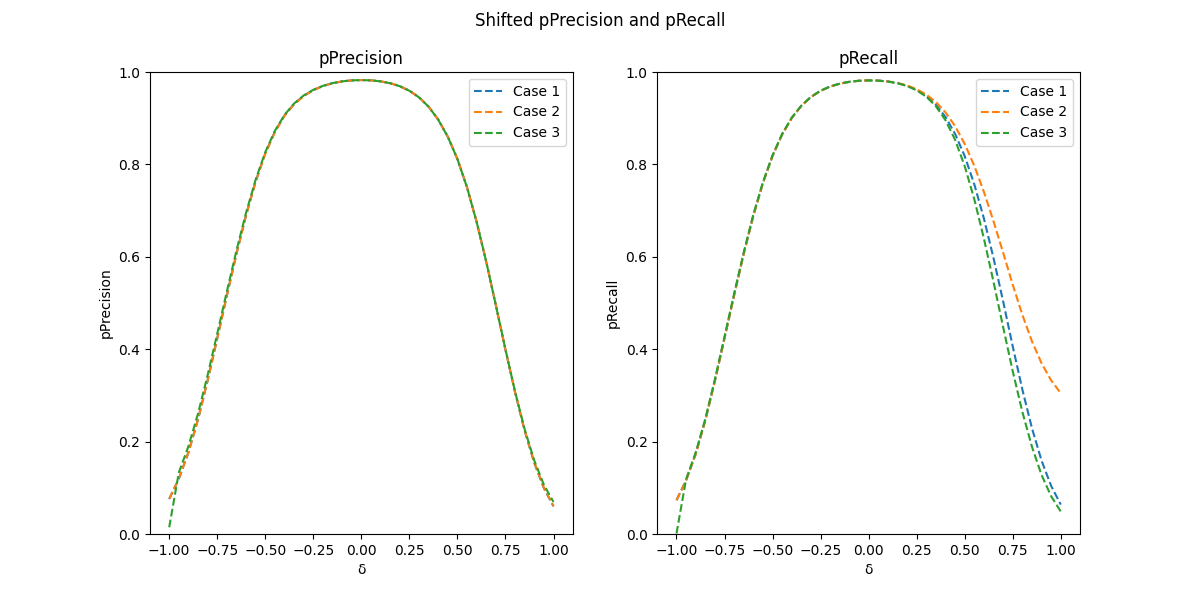
\includegraphics[width=0.8\textwidth]{../images/toyexperiments/outliers/shift_pPrecision_pRecall.png} 
    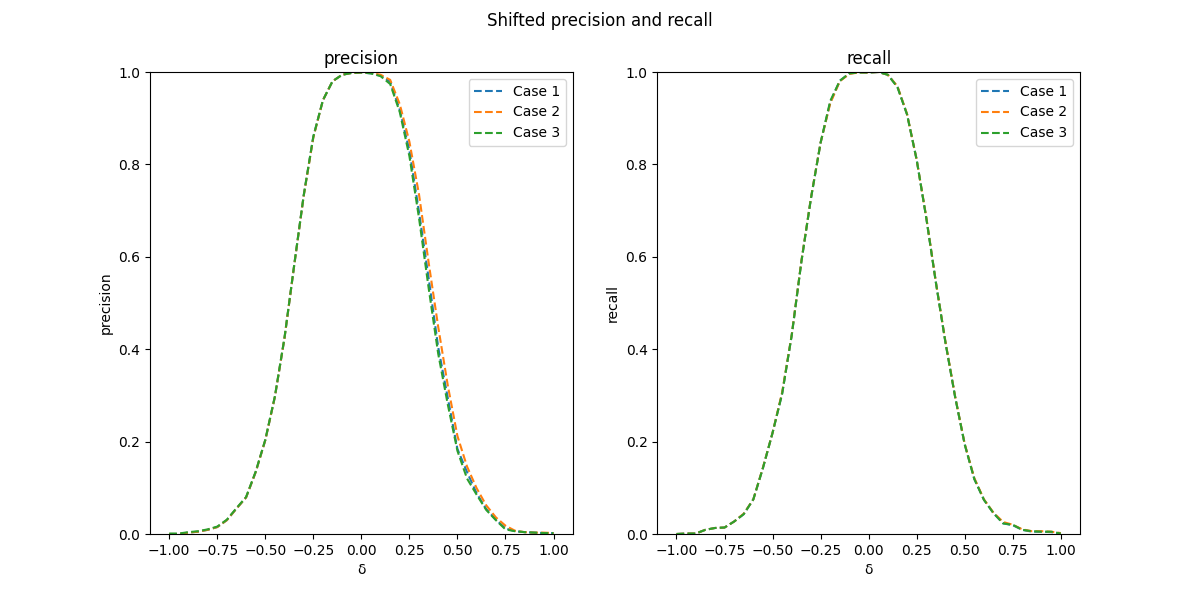
\includegraphics[width=0.8\textwidth]{../images/toyexperiments/outliers/shift_precision_recall.png} 
    \caption{Risultati per la resistenza della probabibilistic precision-recall e della precision-recall coverage alla presenza di outliers nei dati}
\end{figure}

Come per la density e coverage, le due metriche più recenti risultano essere molto robuste alla presenza di outliers nei dati e misurano correttamente la sovrapposizione dei manifold delle due distribuzioni in assenza di shift.
Data la diversa natura delle due metriche, la probabibilistic precision-recall presenta valori più alti quando lo shift è non nullo.

\subsection{Comparazione con implementazioni esistenti e riproduzione delle pr-curves}

Come avevamo anticipato nell'introduzione dei ToyData experiments, abbiamo verificato che le implementazioni presentate nei vari paper presi in esame riportassero risultati conformi a quelli ottenuti con la nostra implementazione.
Per fare ciò, oltre a riprodurre esperimenti simili a quelli presenti nei paper e confrontato i grafici come visto sino ad adesso, abbiamo verificato numericamente che i valori delle metriche fossero effettivamente gli stessi.
Una rapida presa visione del codice sorgente ha permesso di verificare delle differenze implementative che però sono risultate indifferenti se non in termini di complessità computazionale.

Per quanto riguarda le implementazioni di improved precision-recall \cite{2ImprovedPrecisionRecall} i risultati ottenuti sono identici per tutte e tre le distribuzioni di dati presi in analisi.

Per le implementazioni di improved precision-recall e density-coverage \cite{3ReliableFidelityDiversityMetrics} i risultati ottenuti sono identici per tutte e tre le distribuzioni di dati presi in analisi.

Per le implementazioni di probabilistic precision-recall \cite{4ProbabilisticPrecisionRecall} i risultati ottenuti differiscono alla 15esima cifra significativa per tutte e tre le distribuzioni di dati presi in analisi.
Tale differenza non è significativa e può essere attribuita a errori numerici dovuti alla precisione di calcolo delle macchine. Per il calcolo della probabibilistic precision-recall è necessario anche il calcolo della \(\rho(\Phi)\) che è come visto nel capitolo 1 \ref{eq:rho} una media delle \texttt{k}-NN distances,
e nei nostri esperimenti risulta che anche la misura di questa distanza risulta essere equivalente a quella calcolata dalle implementazioni dei papers.

Passiamo ora alla comparazione delle pr-curves. In questo caso le pr-curves riprodotte dipendevano dalla scelta del parametro \texttt{k}, dallo shift fra le due distribuzioni e dallo split del traing set e del test set.
Per i dataset normali con split del 50\% abbiamo ottenuto i seguenti risultati:

\begin{figure}[!ht]
    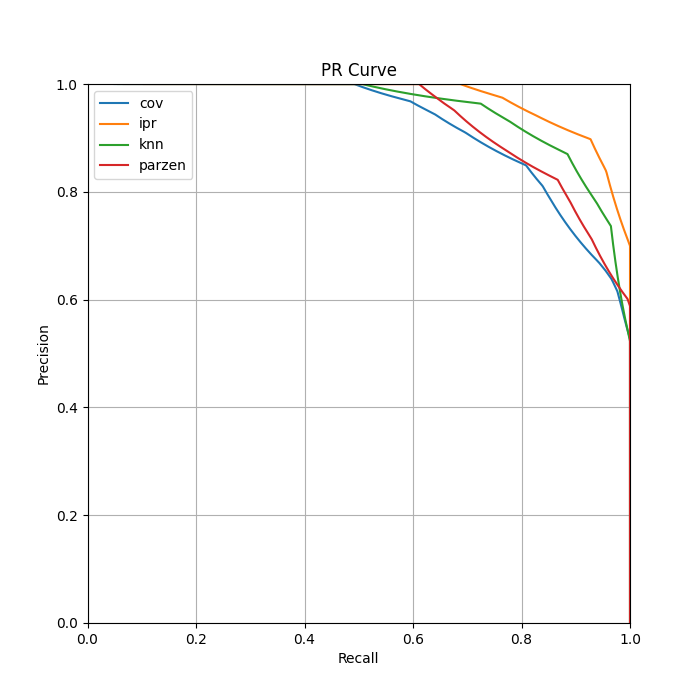
\includegraphics[width=0.5\textwidth]{../images/toyexperiments/prcurves/PRCurve_k4_s1.png} 
    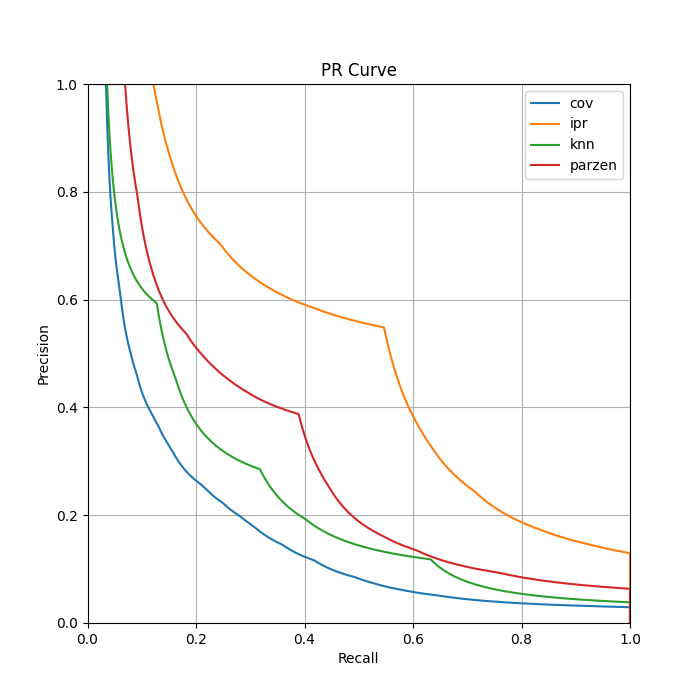
\includegraphics[width=0.5\textwidth]{../images/toyexperiments/prcurves/PRCurve_k4_s3.png}
    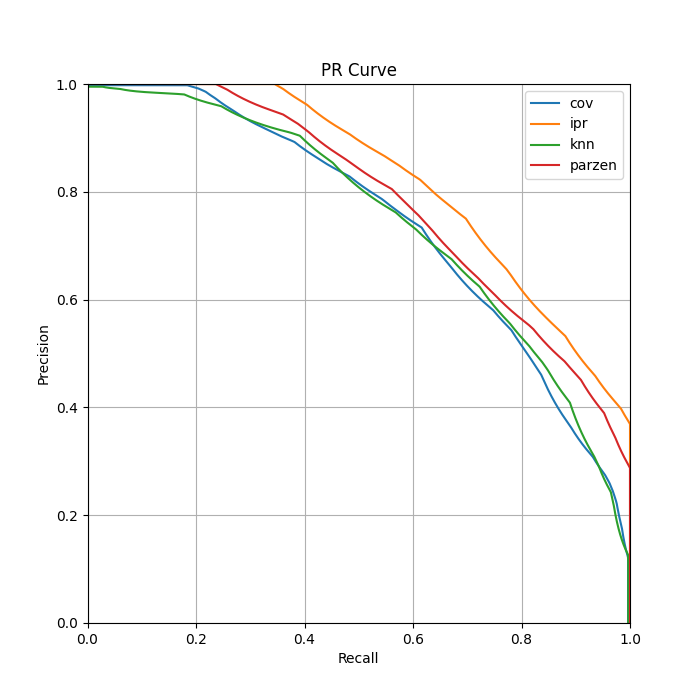
\includegraphics[width=0.5\textwidth]{../images/toyexperiments/prcurves/PRCurve_ksqrt_s1.png} 
    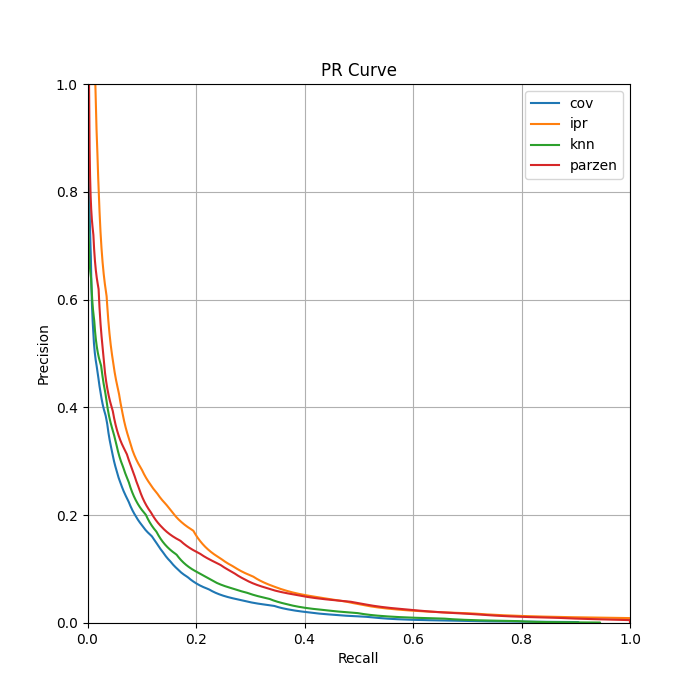
\includegraphics[width=0.5\textwidth]{../images/toyexperiments/prcurves/PRCurve_ksqrt_s3.png}
    \caption{Risultati per le pr-curves per dataset normali con split del 50\%} 
\end{figure}


Per i dataset normali senza split abbiamo ottenuto i seguenti risultati:

\begin{figure}[!ht]
    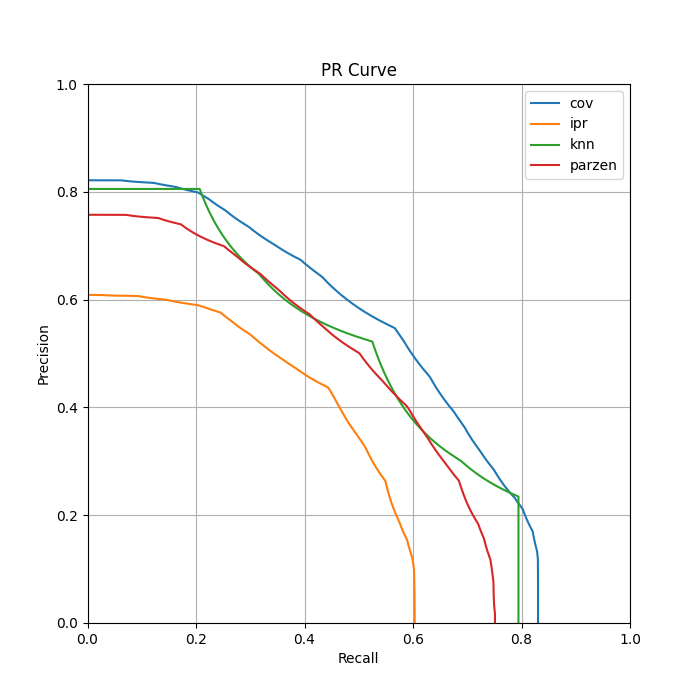
\includegraphics[width=0.5\textwidth]{../images/toyexperiments/prcurves/PRCurve_nosplit_k4_s1.png}
    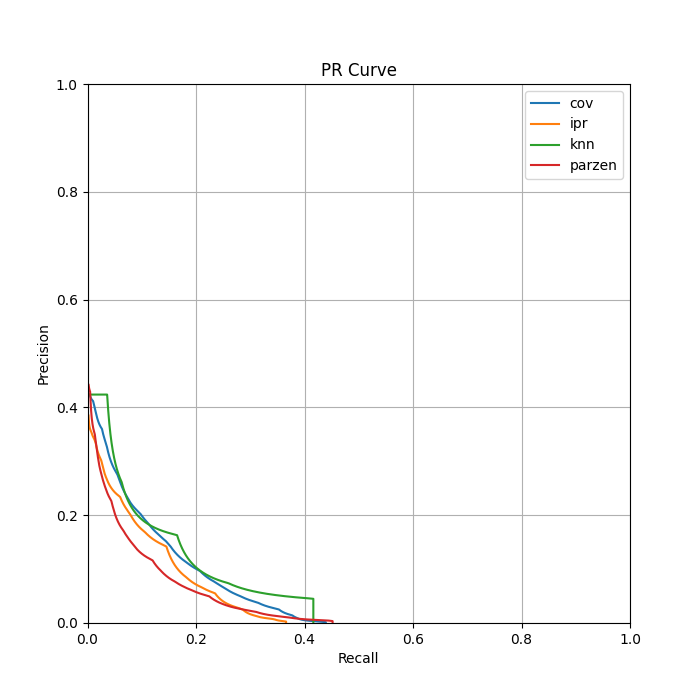
\includegraphics[width=0.5\textwidth]{../images/toyexperiments/prcurves/PRCurve_nosplit_k4_s3.png}
    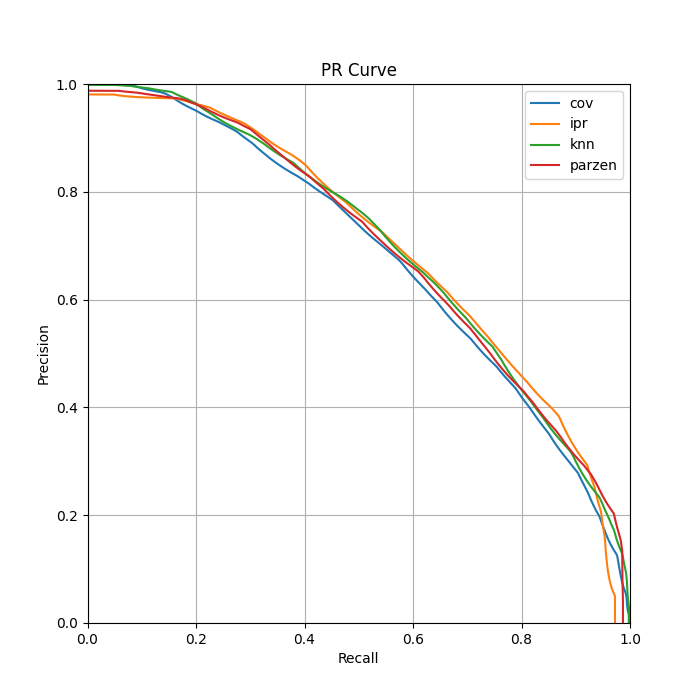
\includegraphics[width=0.5\textwidth]{../images/toyexperiments/prcurves/PRCurve_nosplit_ksqrt_s1.png}
    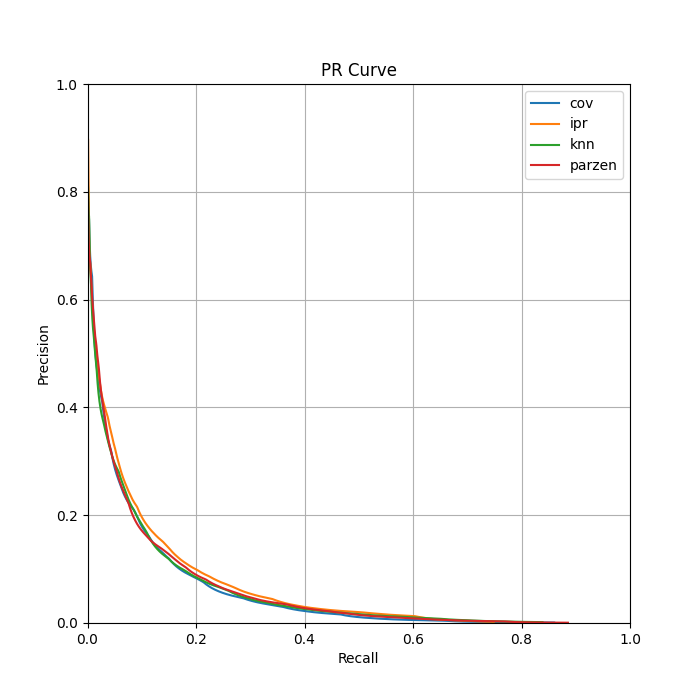
\includegraphics[width=0.5\textwidth]{../images/toyexperiments/prcurves/PRCurve_nosplit_ksqrt_s3.png}
    \caption{Risultati per le pr-curves per dataset normali senza split}
\end{figure}

Anche in questo caso i risultati ottenuti sono conformi a quelli attesi e presenti nei paper. Le conclusioni che si possono trarre sono pertanto le stesse di quelle presenti nei paper, vale a dire che si nota una maggiore stabilità delle pr-curves in presenza di uno split del dataset e con \texttt{k = \(\sqrt{|\Phi|}\)}.

\section{Risultati degli esperimenti su dataset reali}

\subsection{Butterflies}
\label{subsec:res-butterflies}

Prima di condurre gli esperimenti per identificare se le metriche possano operare correttamente da filtro per la selezione di dati generati di alta qualità, abbiamo condotto degli esperimenti preliminari per studiare il dominio in cui avrebbero operato le metriche.
In particolare abbiamo analizzato le kde delle divese caratterristiche proposte per le distanze inter e intra set. L'obbiettivo era quello di verificare che tali caratterristiche fossero sufficientemente descrittive per poter distinguere dati generati di alta qualità da dati generati di bassa qualità.
I risultati ottenuti sono i seguenti:

\begin{figure}[!ht]
    \centering
    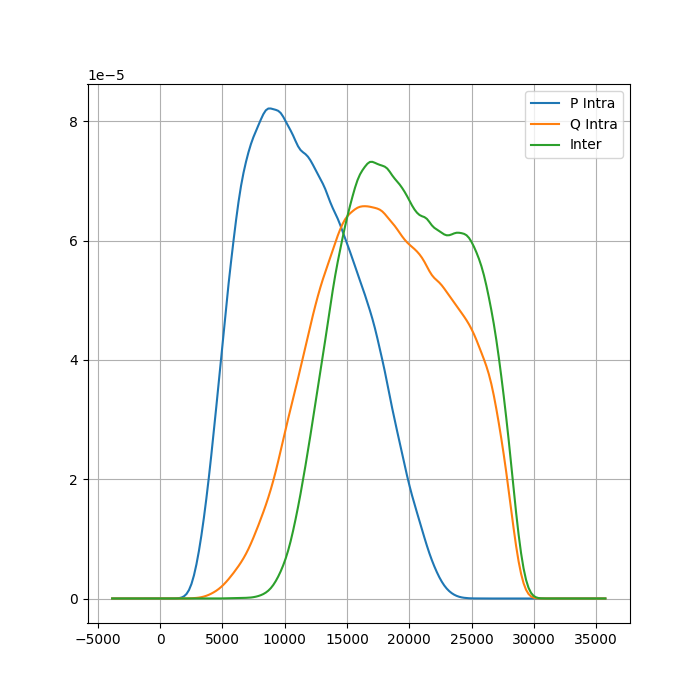
\includegraphics[width=0.3\textwidth]{../images/realworldexperiments/butterflies/kde/kde_grayscale_histogram.png}
    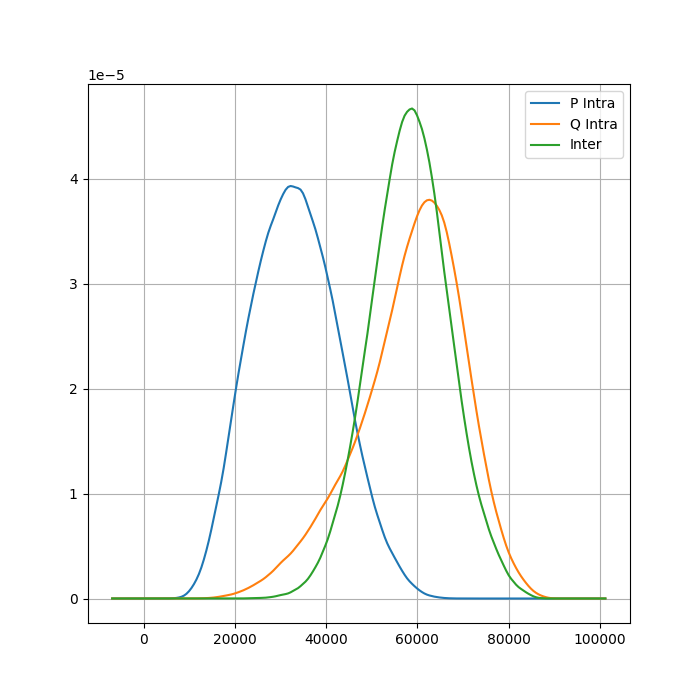
\includegraphics[width=0.3\textwidth]{../images/realworldexperiments/butterflies/kde/kde_hsv_histogram.png}
    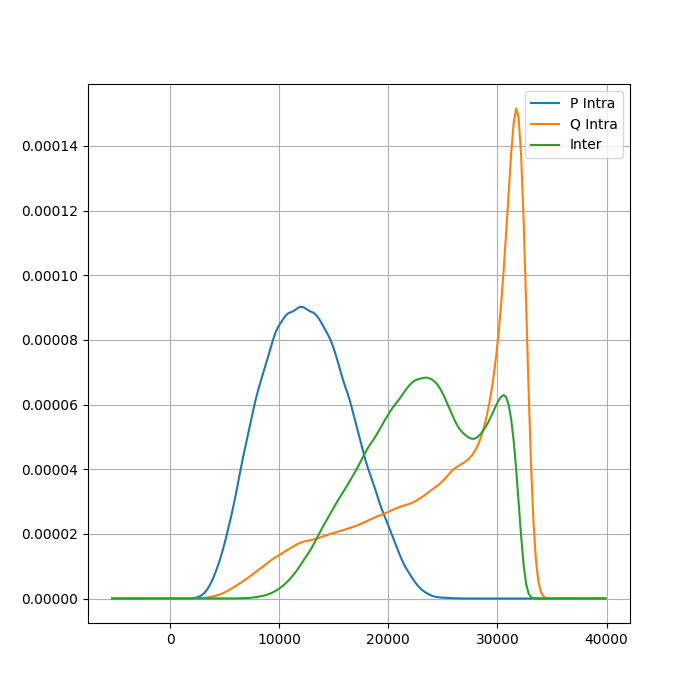
\includegraphics[width=0.3\textwidth]{../images/realworldexperiments/butterflies/kde/kde_hue_histogram.png}
\end{figure}
\begin{figure}[!ht]
    \centering
    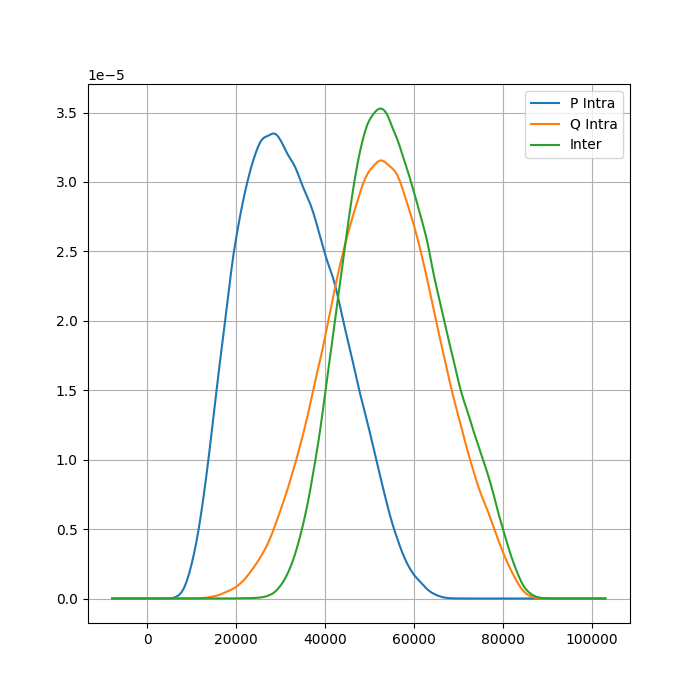
\includegraphics[width=0.3\textwidth]{../images/realworldexperiments/butterflies/kde/kde_rgb_histogram.png}
    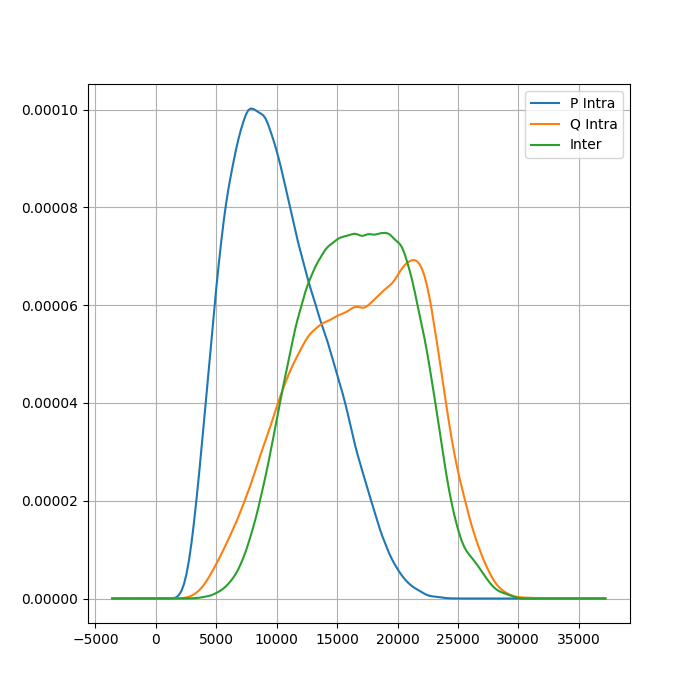
\includegraphics[width=0.3\textwidth]{../images/realworldexperiments/butterflies/kde/kde_saturation_histogram.png}
    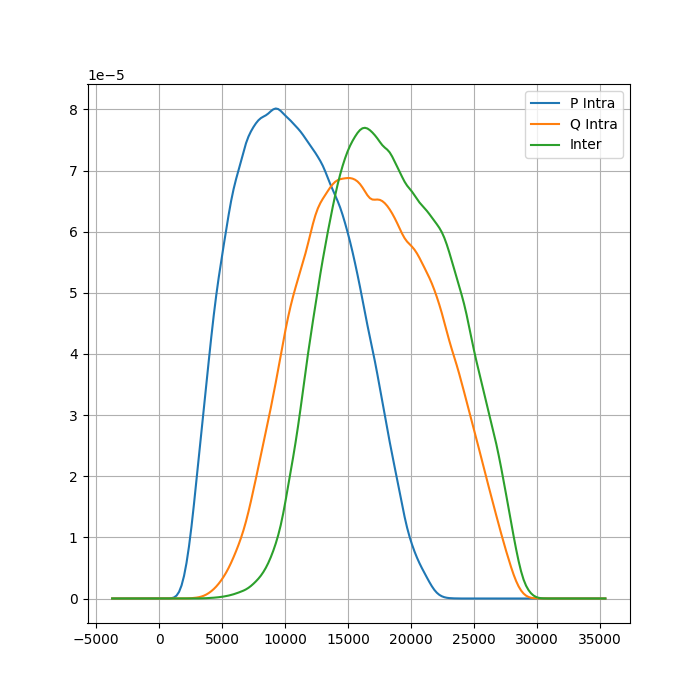
\includegraphics[width=0.3\textwidth]{../images/realworldexperiments/butterflies/kde/kde_value_histogram.png}
    \caption{l'ordine delle immagini da sinistra a destra e dall'alto in basso è: grayscale, hsv, hue, rgb, saturation, value}
\end{figure}

L'analisi delle Kernel Density Estimation (KDE) applicata alle distanze intra-set per i campioni reali e quelli generati evidenzia una limitata sovrapposizione tra le distribuzioni. Le distanze intra-set dei dati reali si concentrano, come ci si potrebbe aspettare intorno a valori più bassi, mentre quelle dei dati generati mostrano una maggiore dispersione, con una tendenza verso distanze più elevate. Questo comportamento implica che i campioni generati, anche quelli più vicini al manifold dei dati reali, difficilmente raggiungono la stessa compattezza dei campioni reali.

Per ogni tipo di istogramma analizzato, sono stati selezionati i 5 falsi positivi (immagini generate che ricadono nel manifold dei dati reali) con le distanze più elevate dai dati reali e i 5 veri positivi (immagini generate correttamente che ricadono sotto il manifold dei dati reali) con le distanze minori. Questi sono stati confrontati con le rispettive immagini reali più vicine, per un totale di 20 immagini per ogni istogramma. 
I risultati sono nella figura \ref{fig:realworldexperiments-butterflies} che segue.

\begin{figure}[!ht]
    \label{fig:realworldexperiments-butterflies}
    \centering
    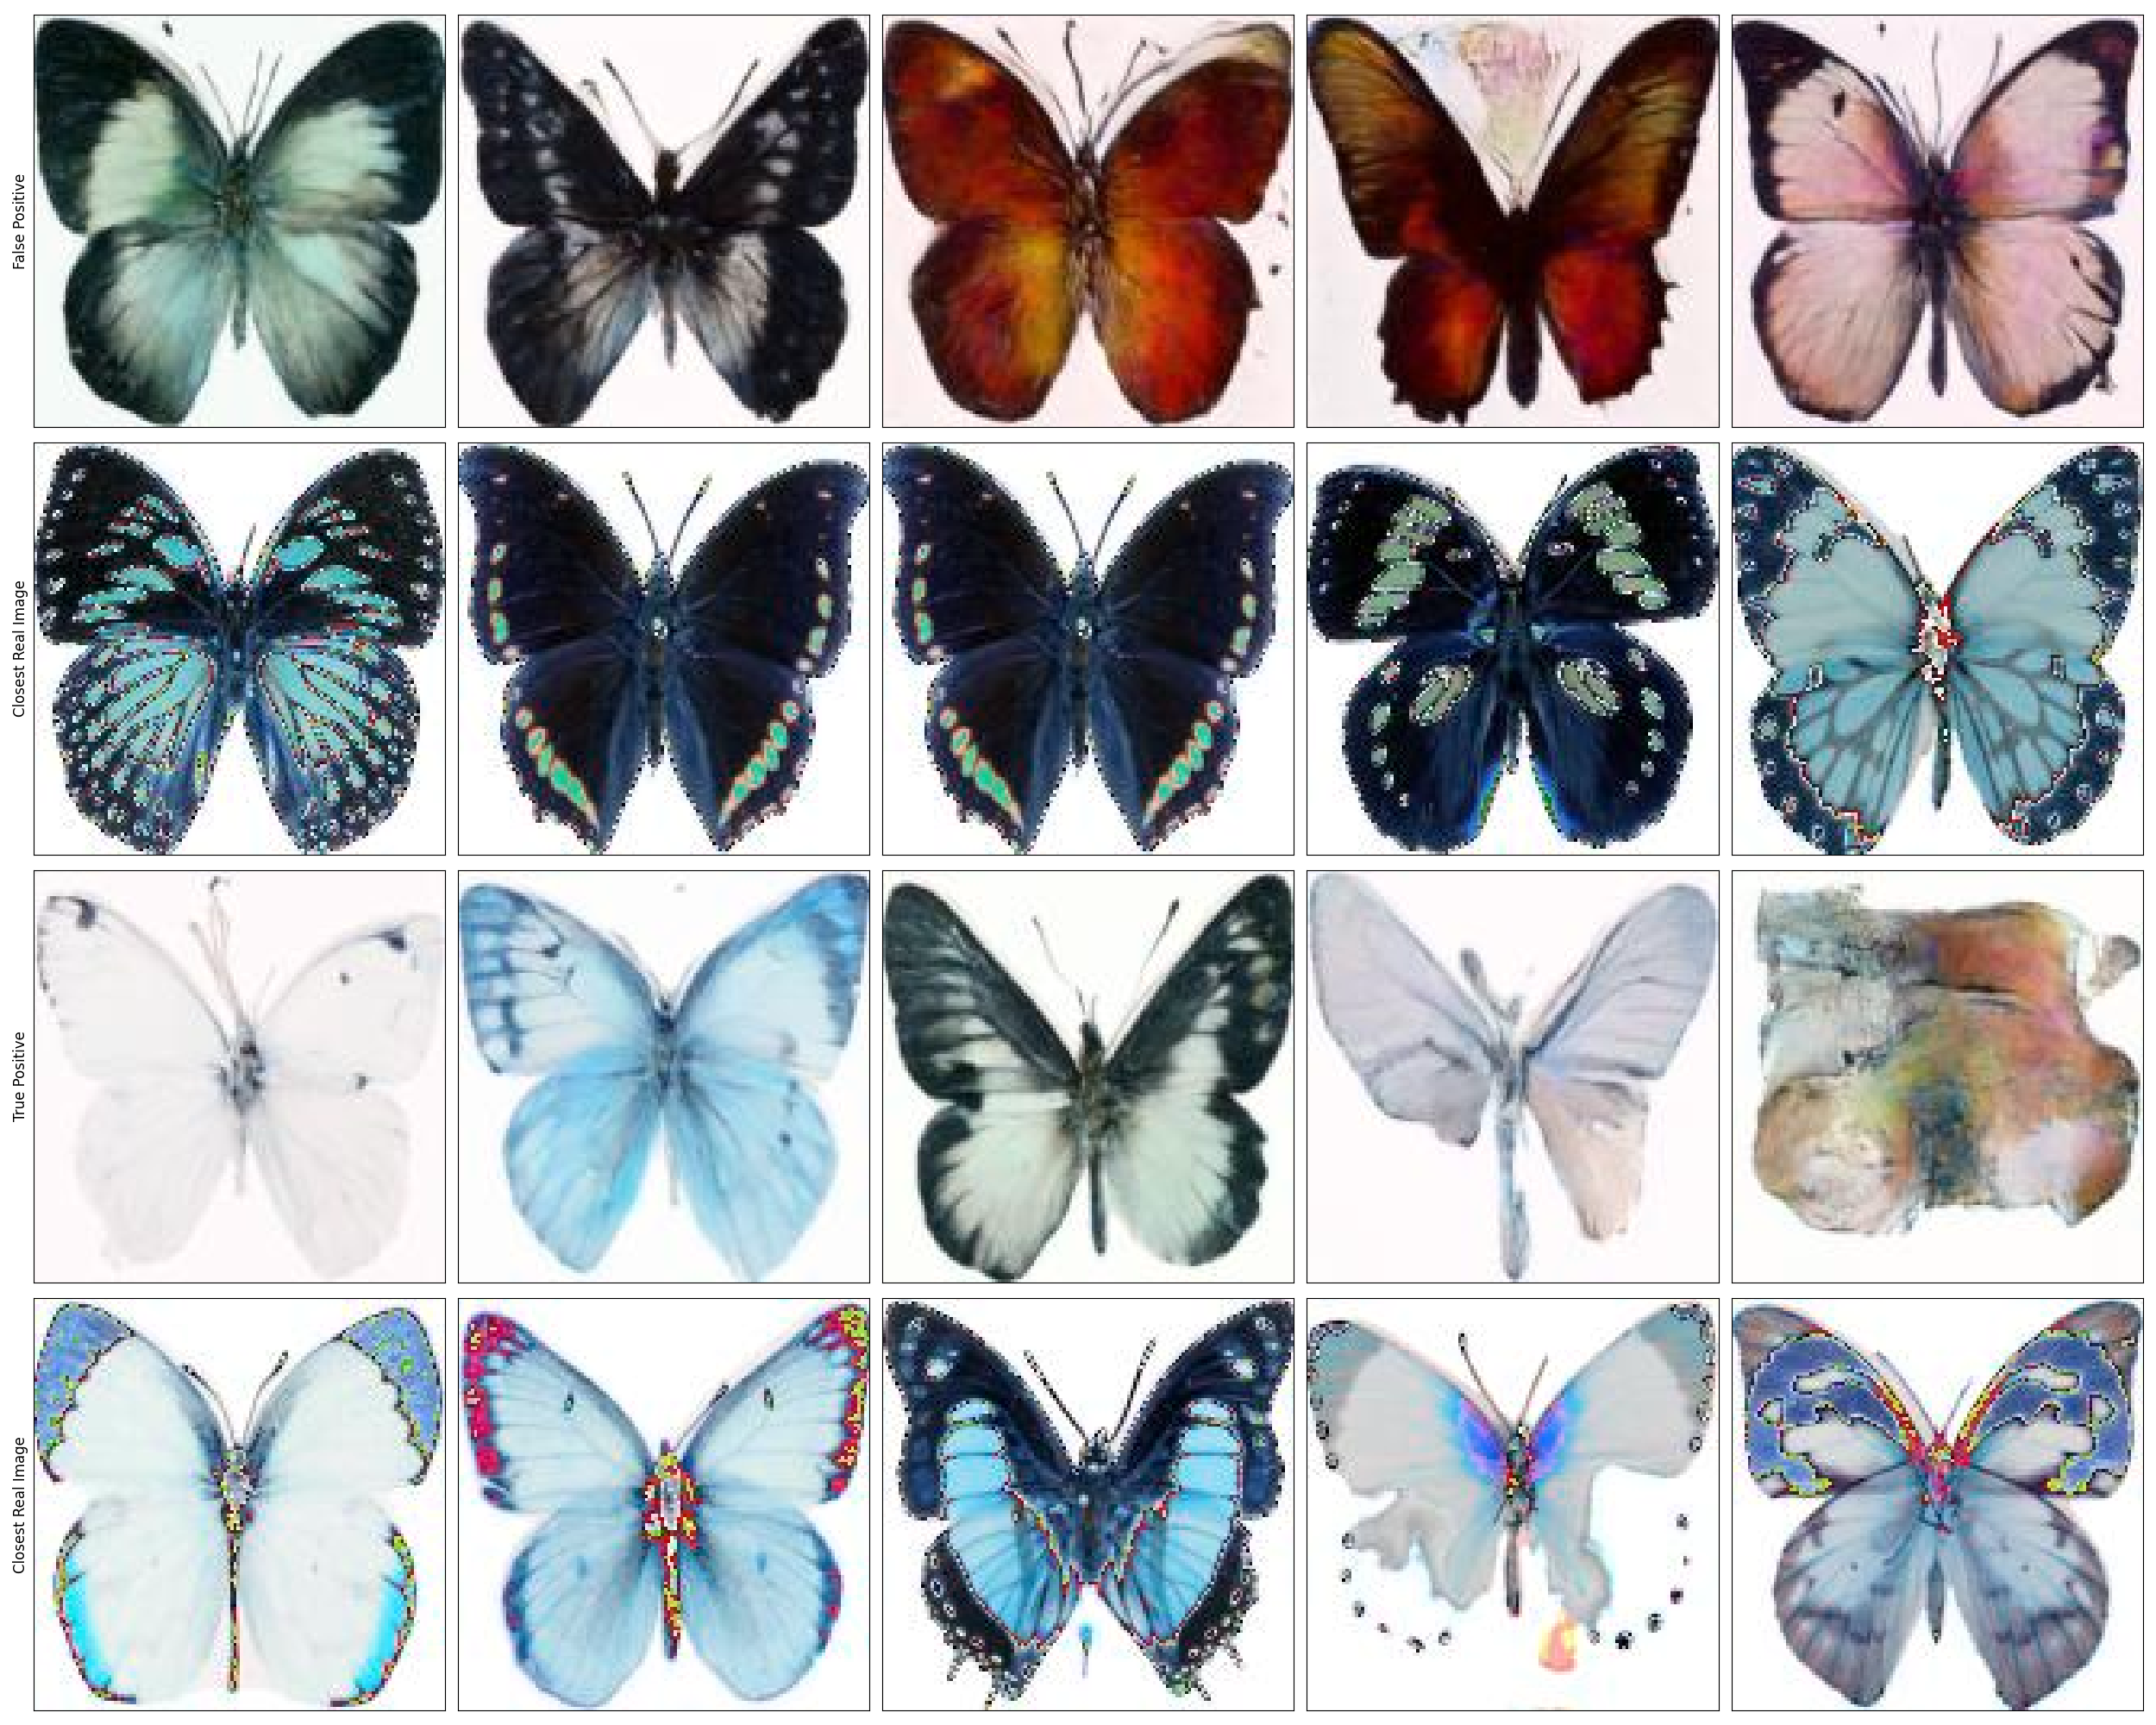
\includegraphics[width=0.45\textwidth]{../images/realworldexperiments/butterflies/examples/fp_grayscale_histogram.png}
    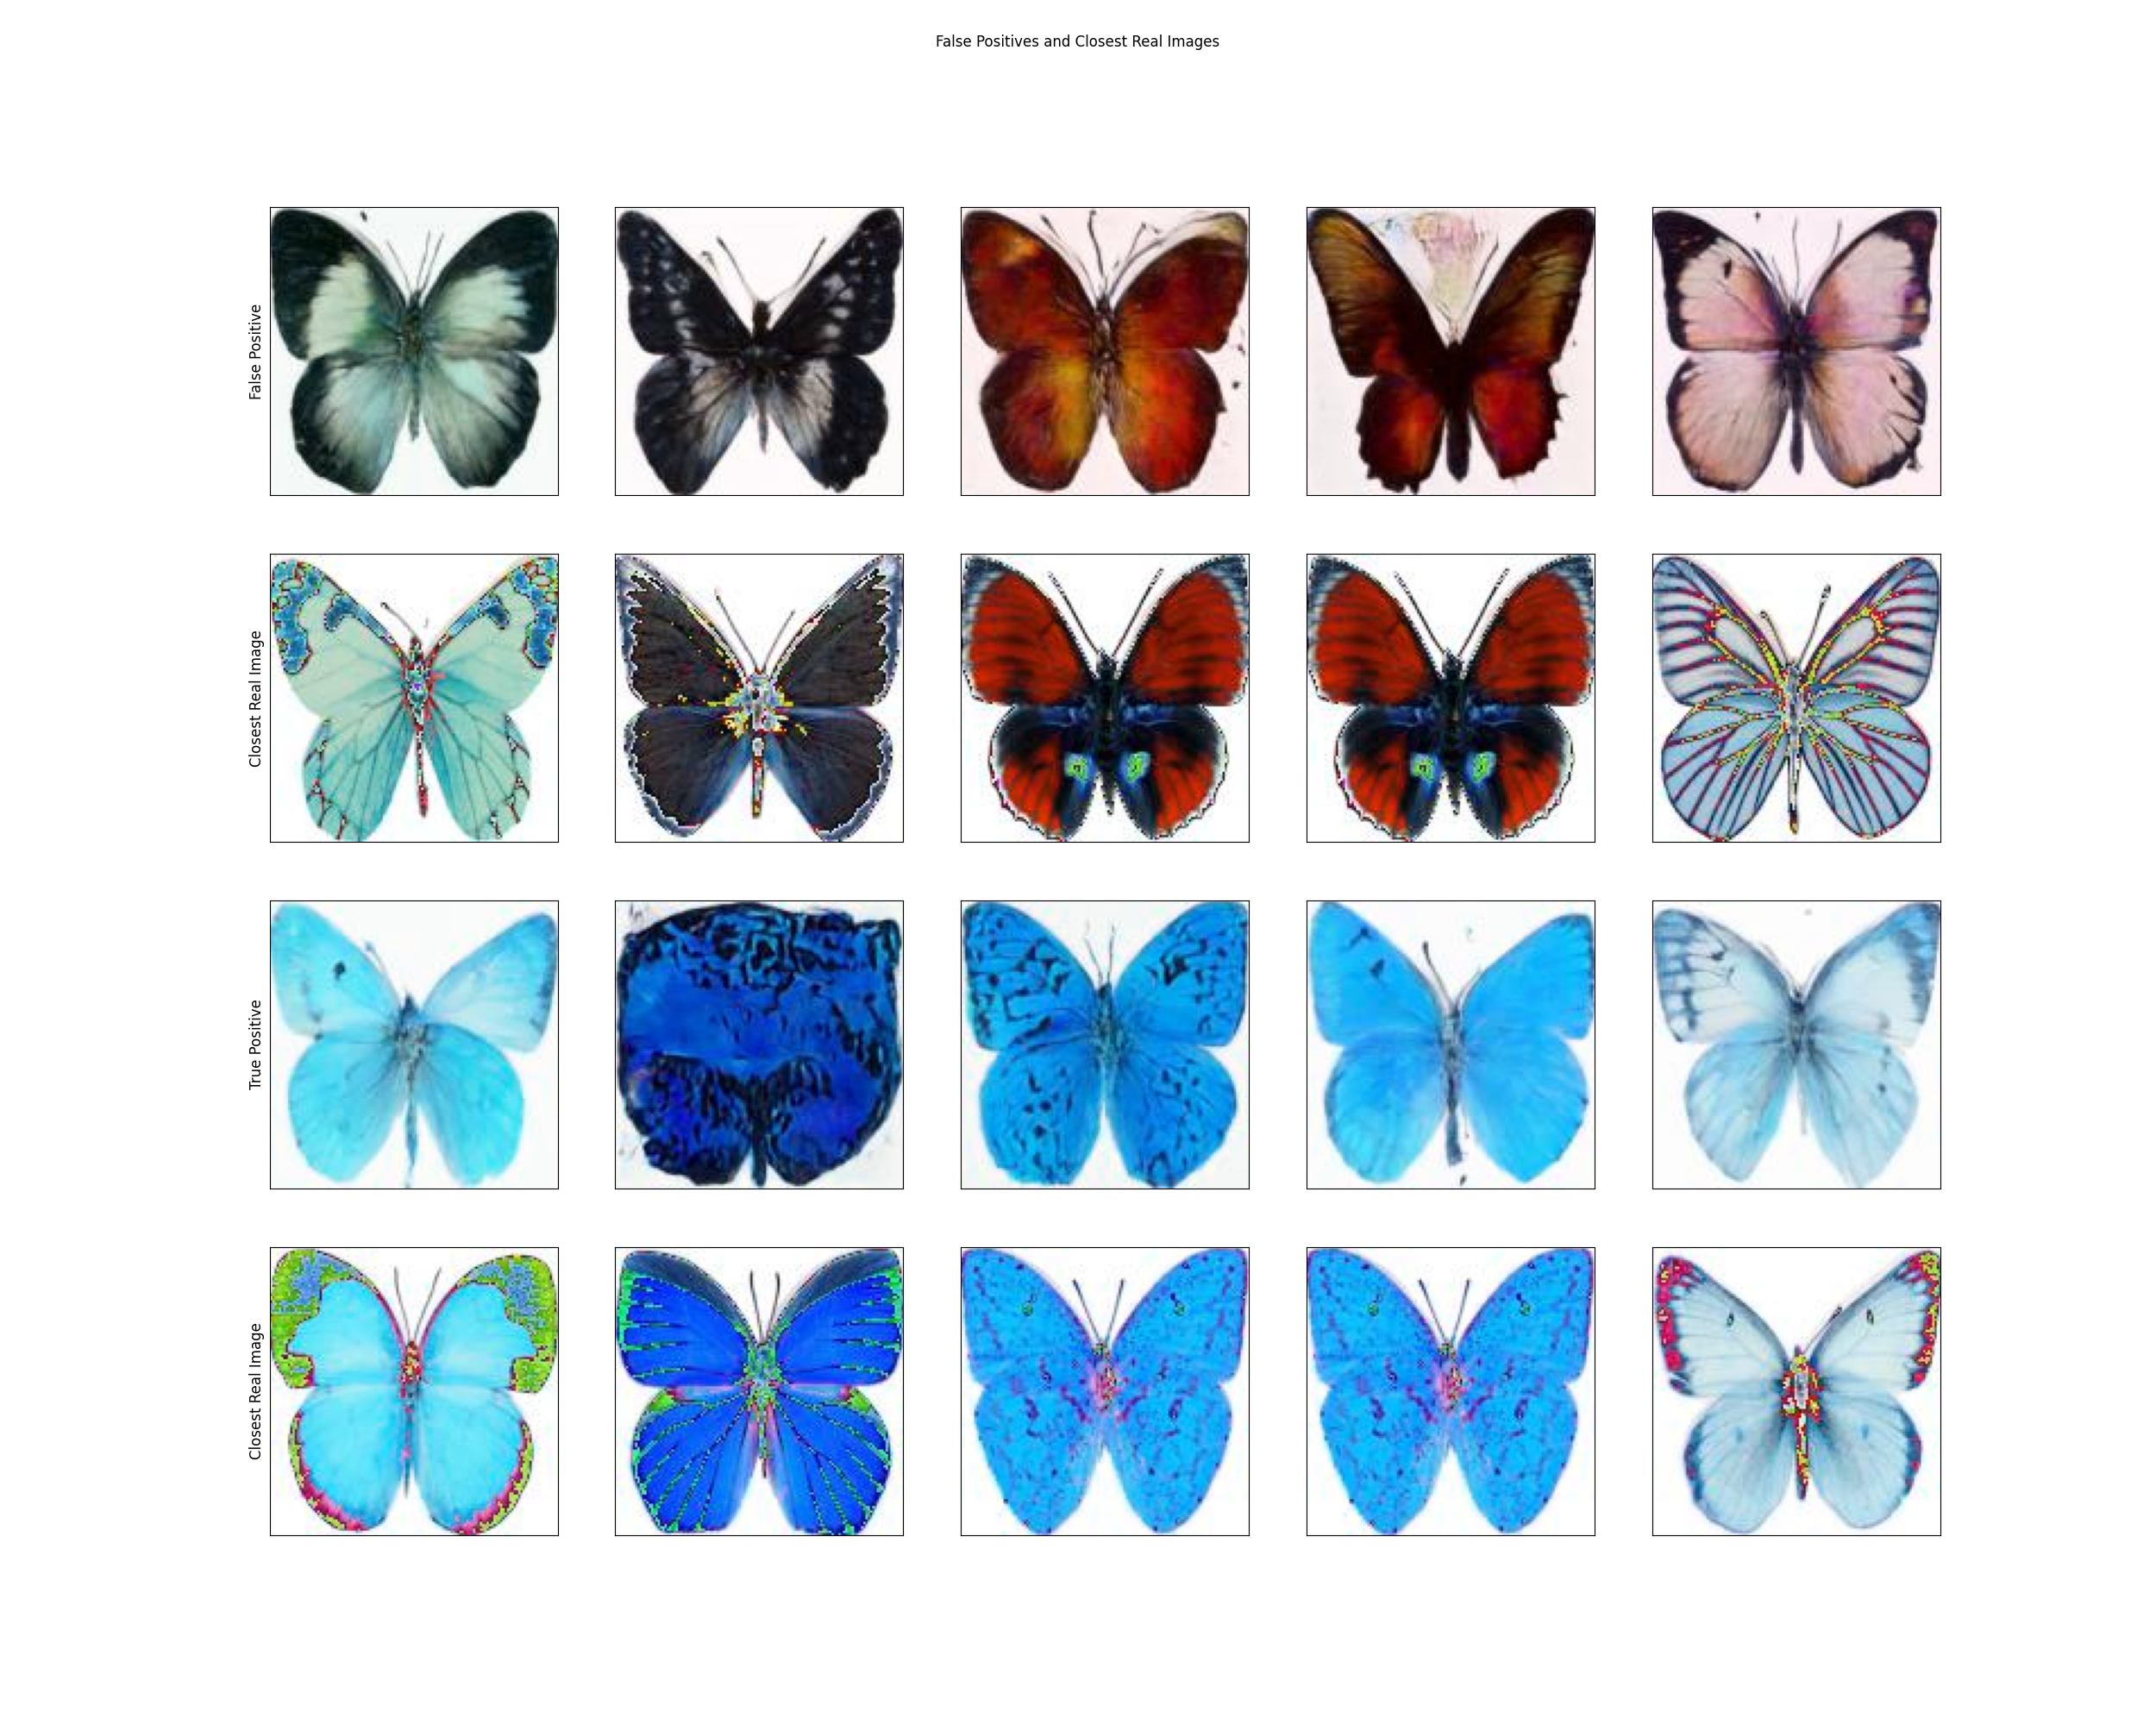
\includegraphics[width=0.45\textwidth]{../images/realworldexperiments/butterflies/examples/fp_hsv_histogram.png}
    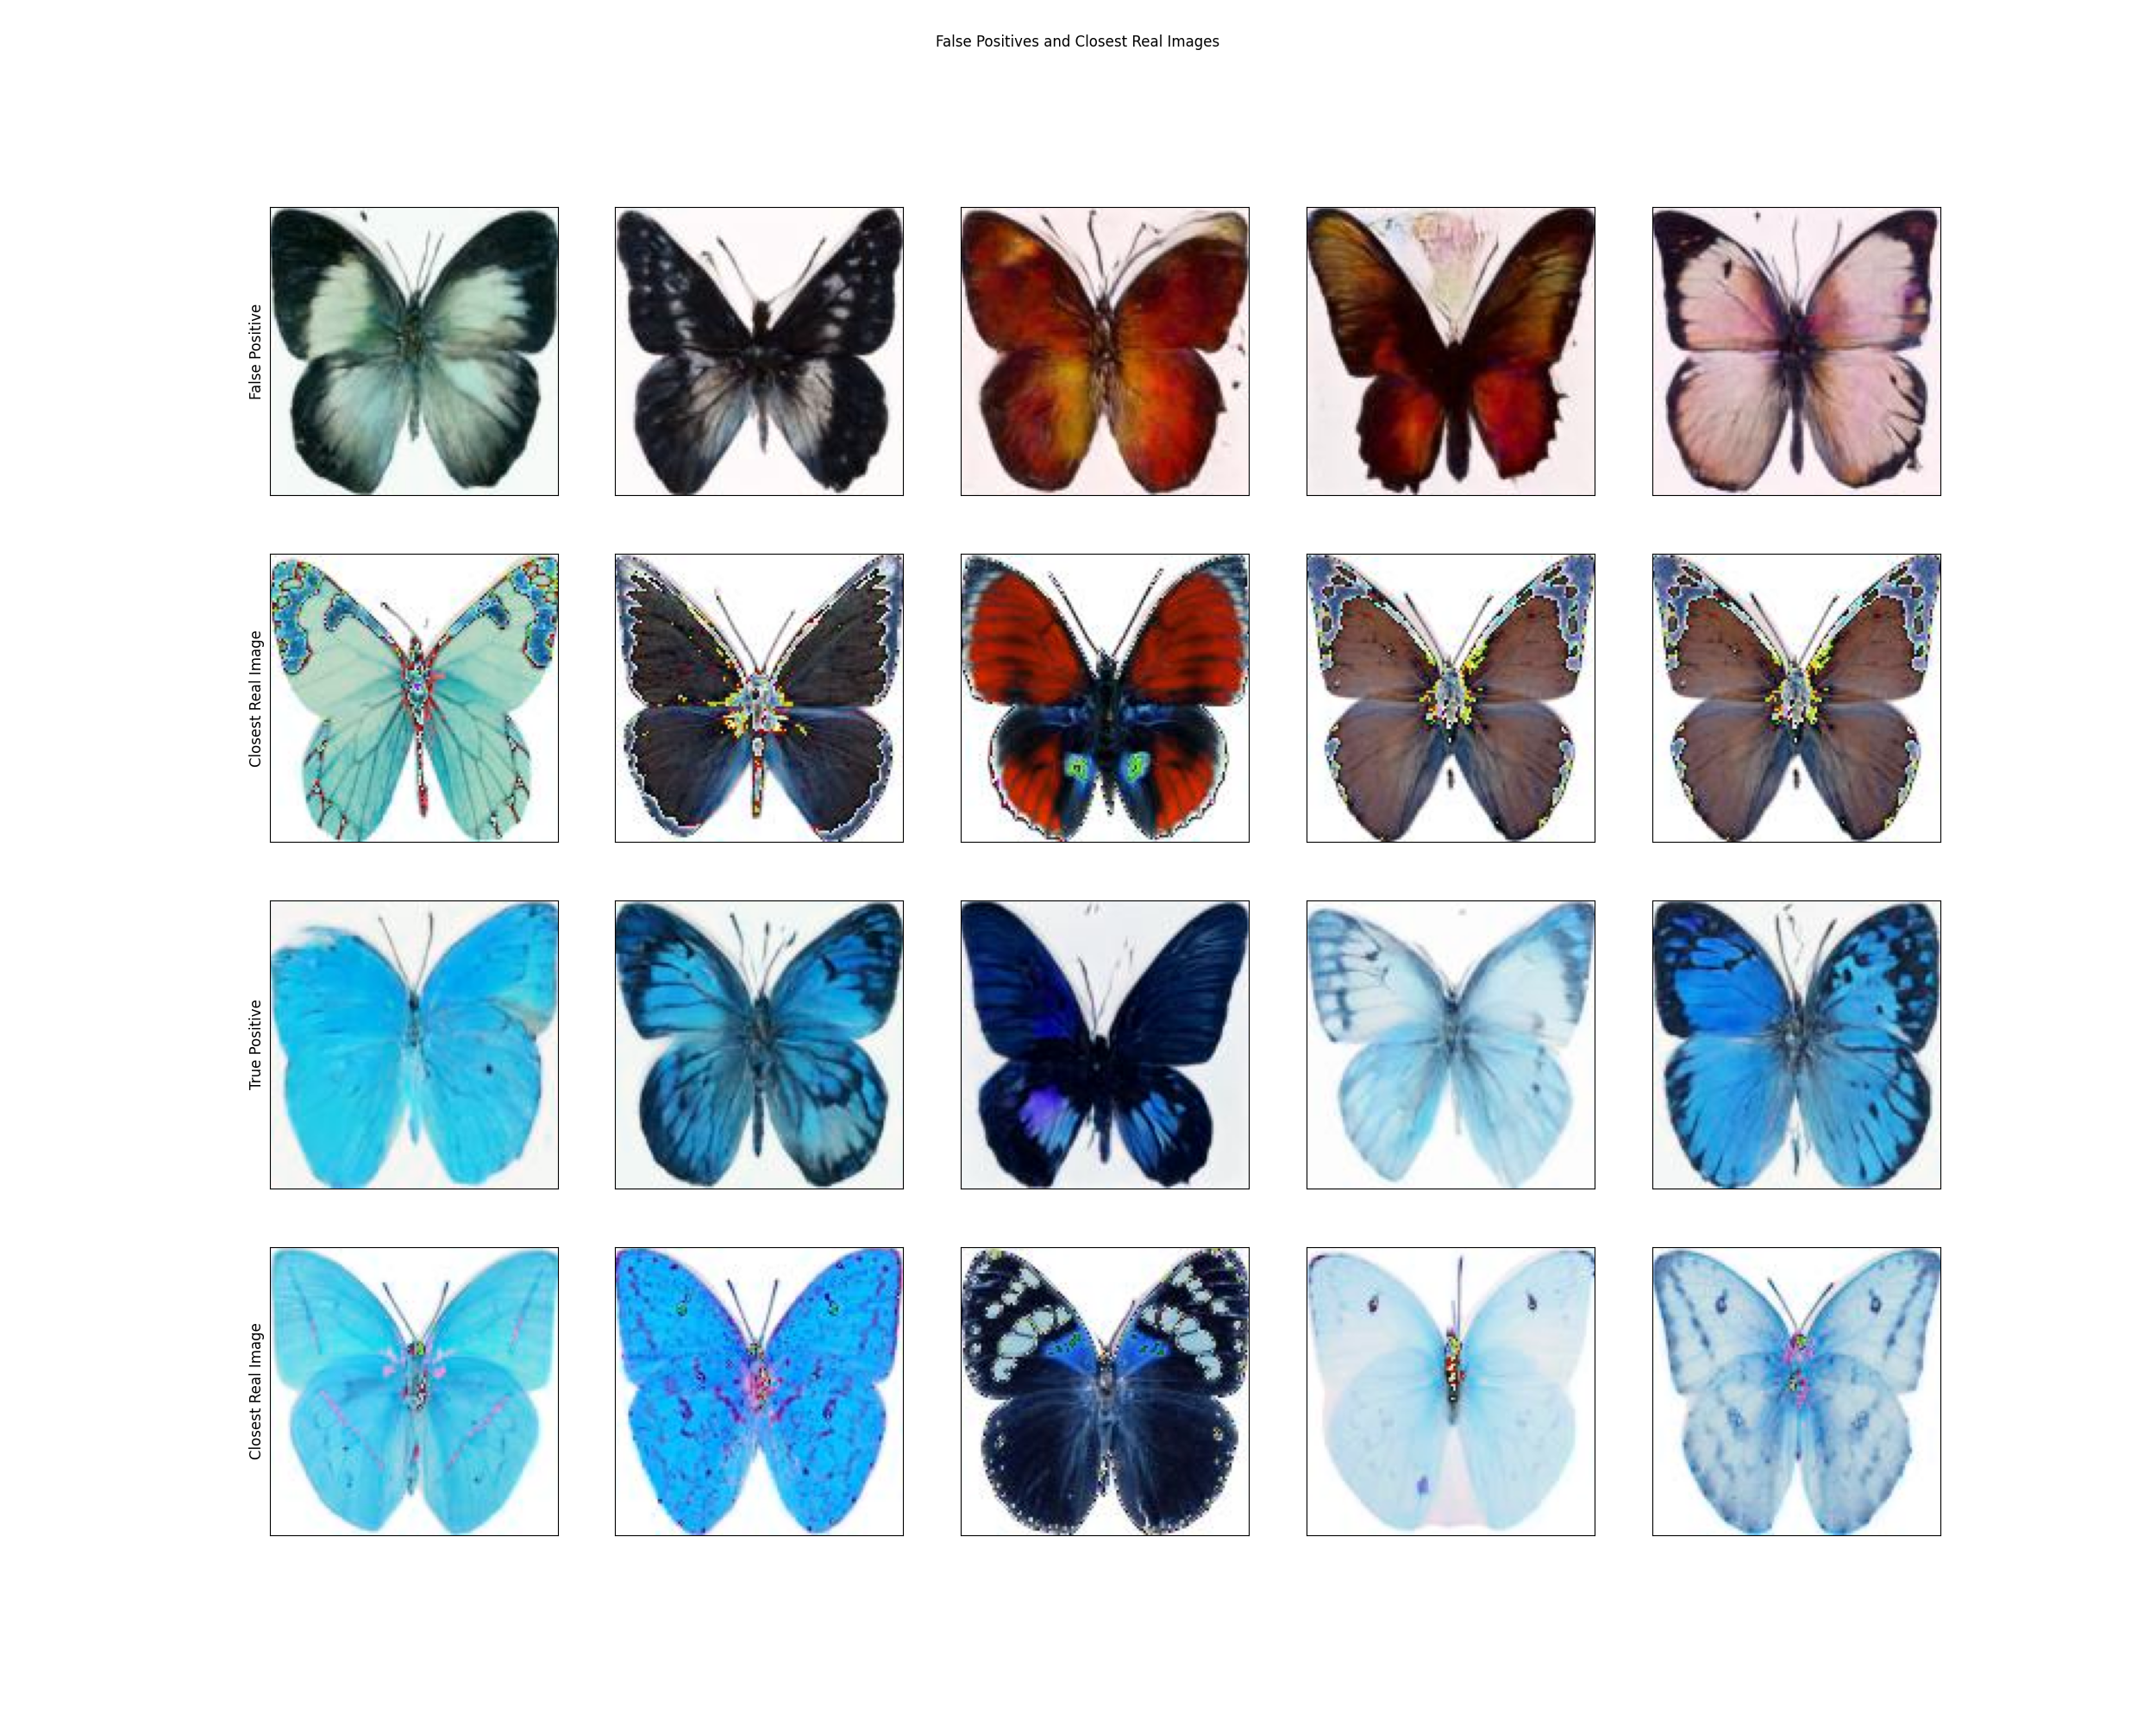
\includegraphics[width=0.45\textwidth]{../images/realworldexperiments/butterflies/examples/fp_hue_histogram.png}
    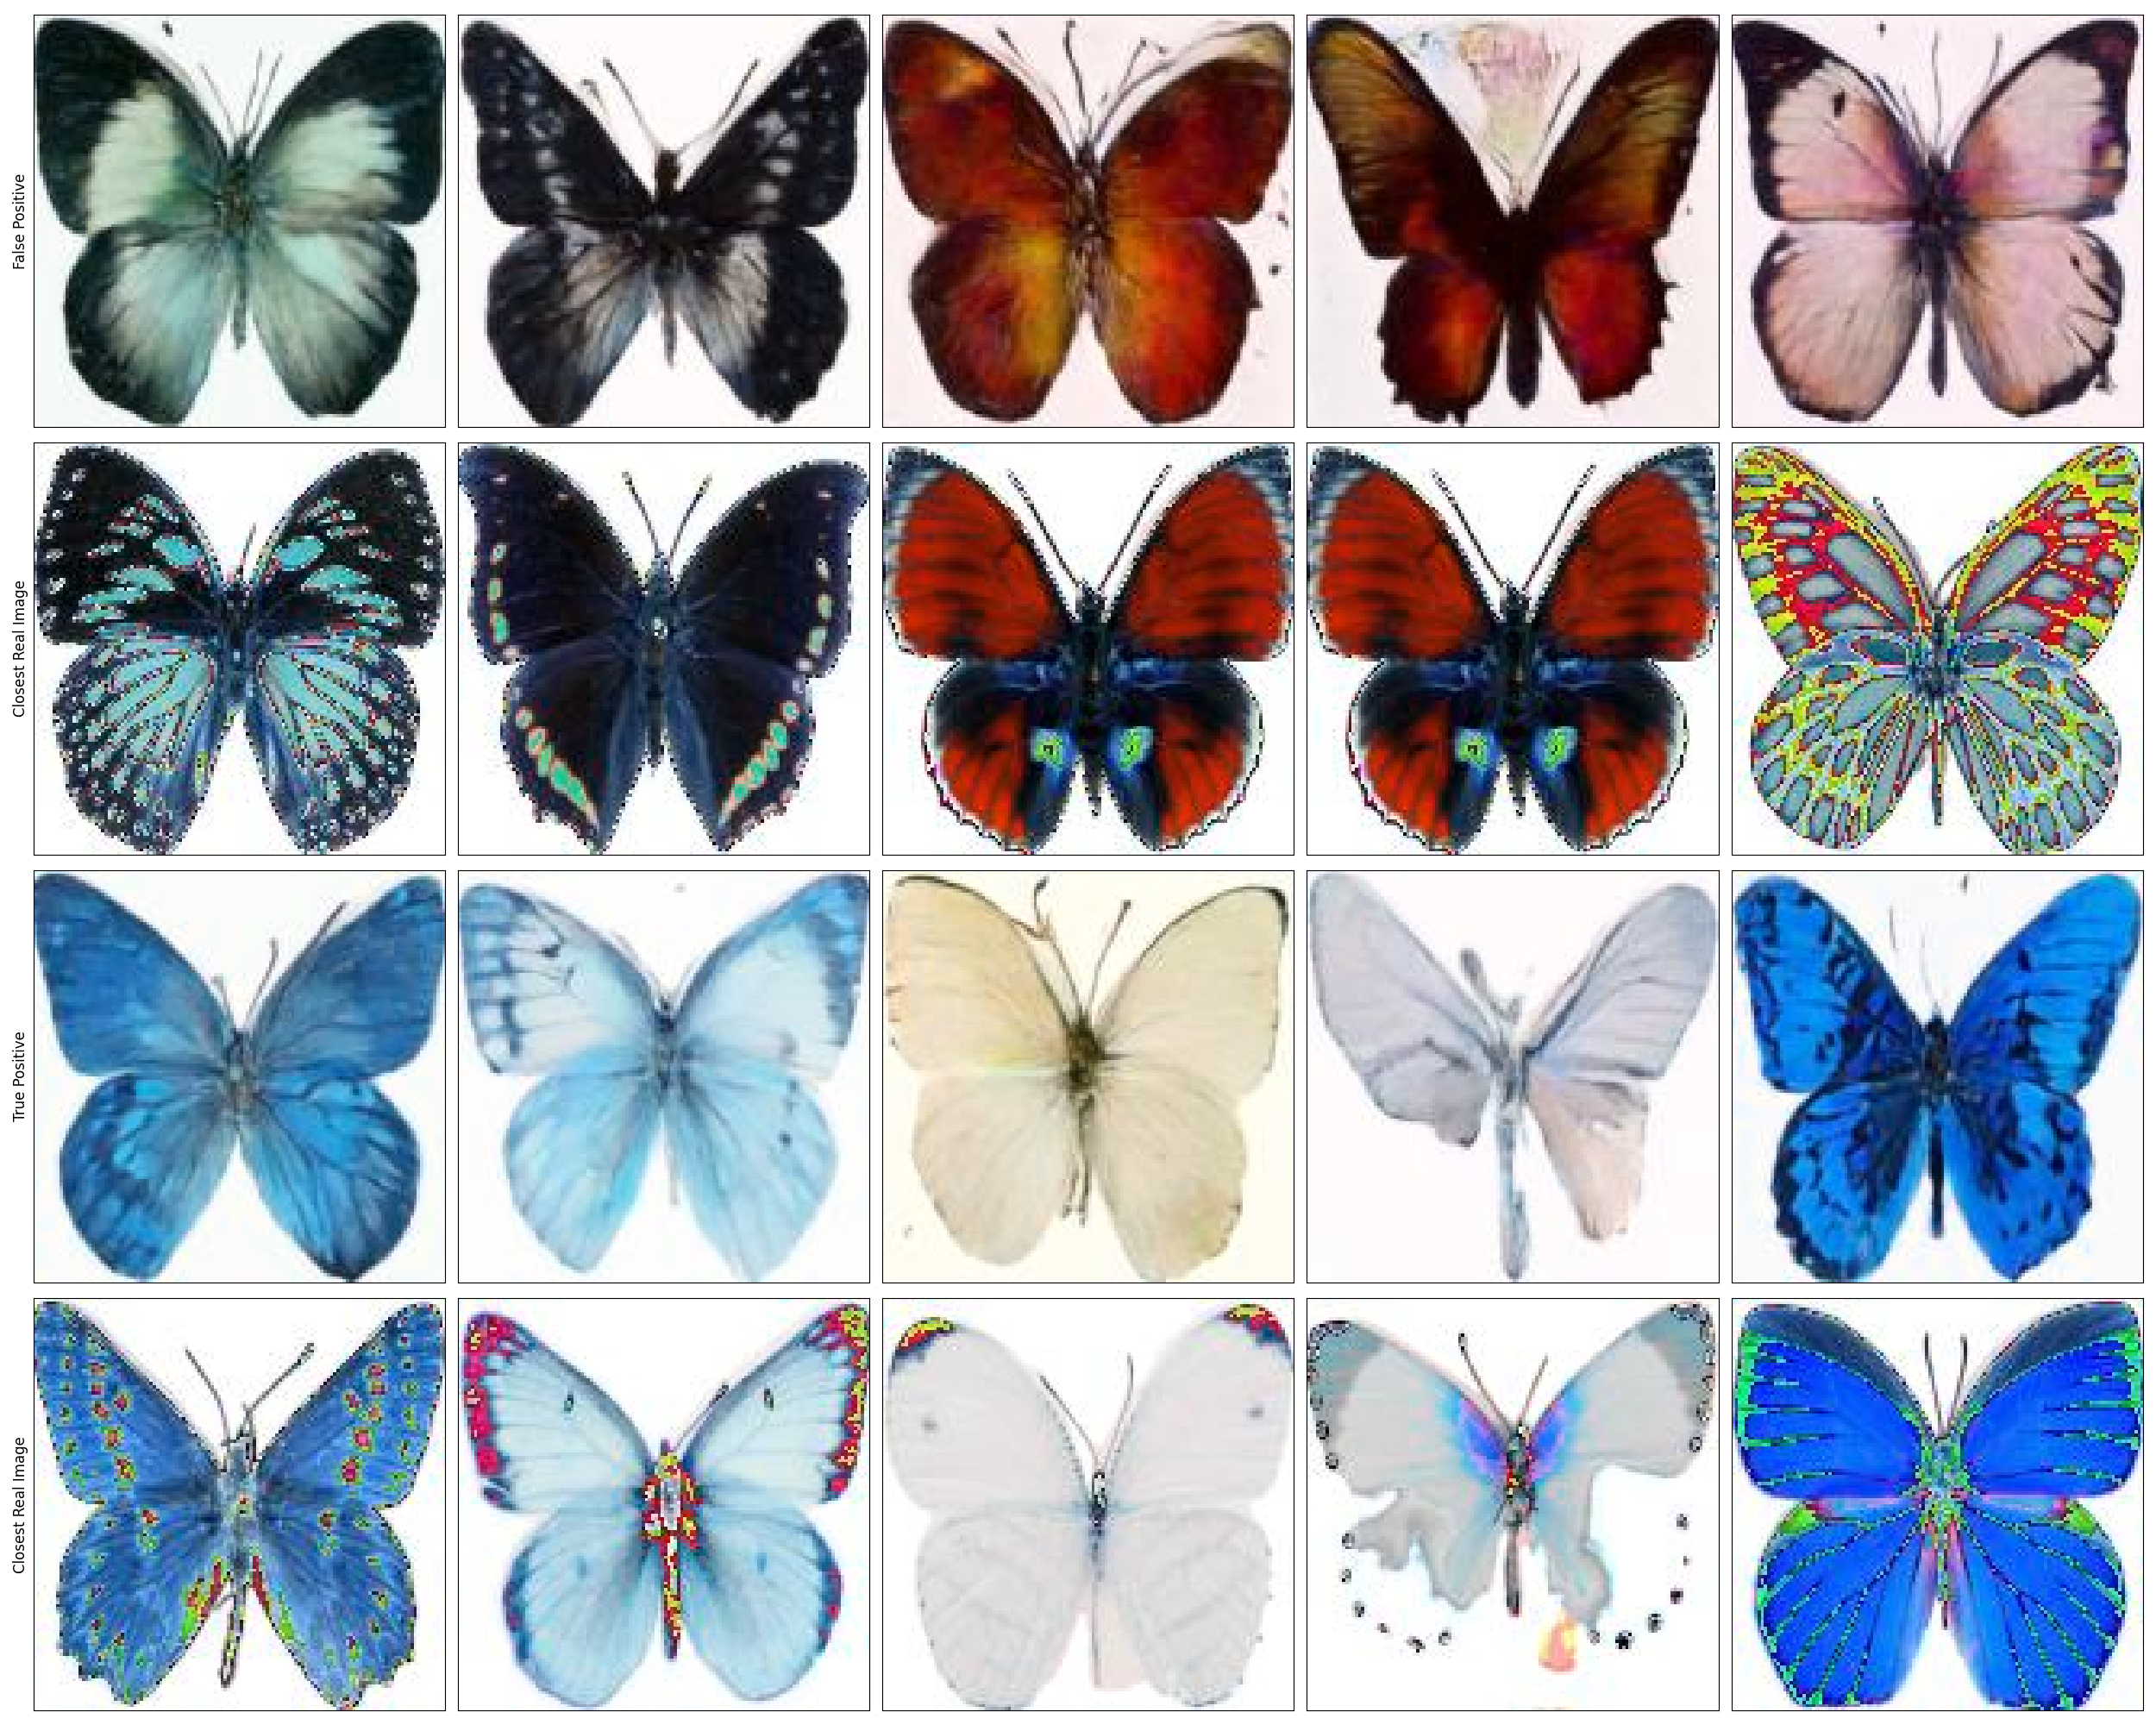
\includegraphics[width=0.45\textwidth]{../images/realworldexperiments/butterflies/examples/fp_rgb_histogram.png}
    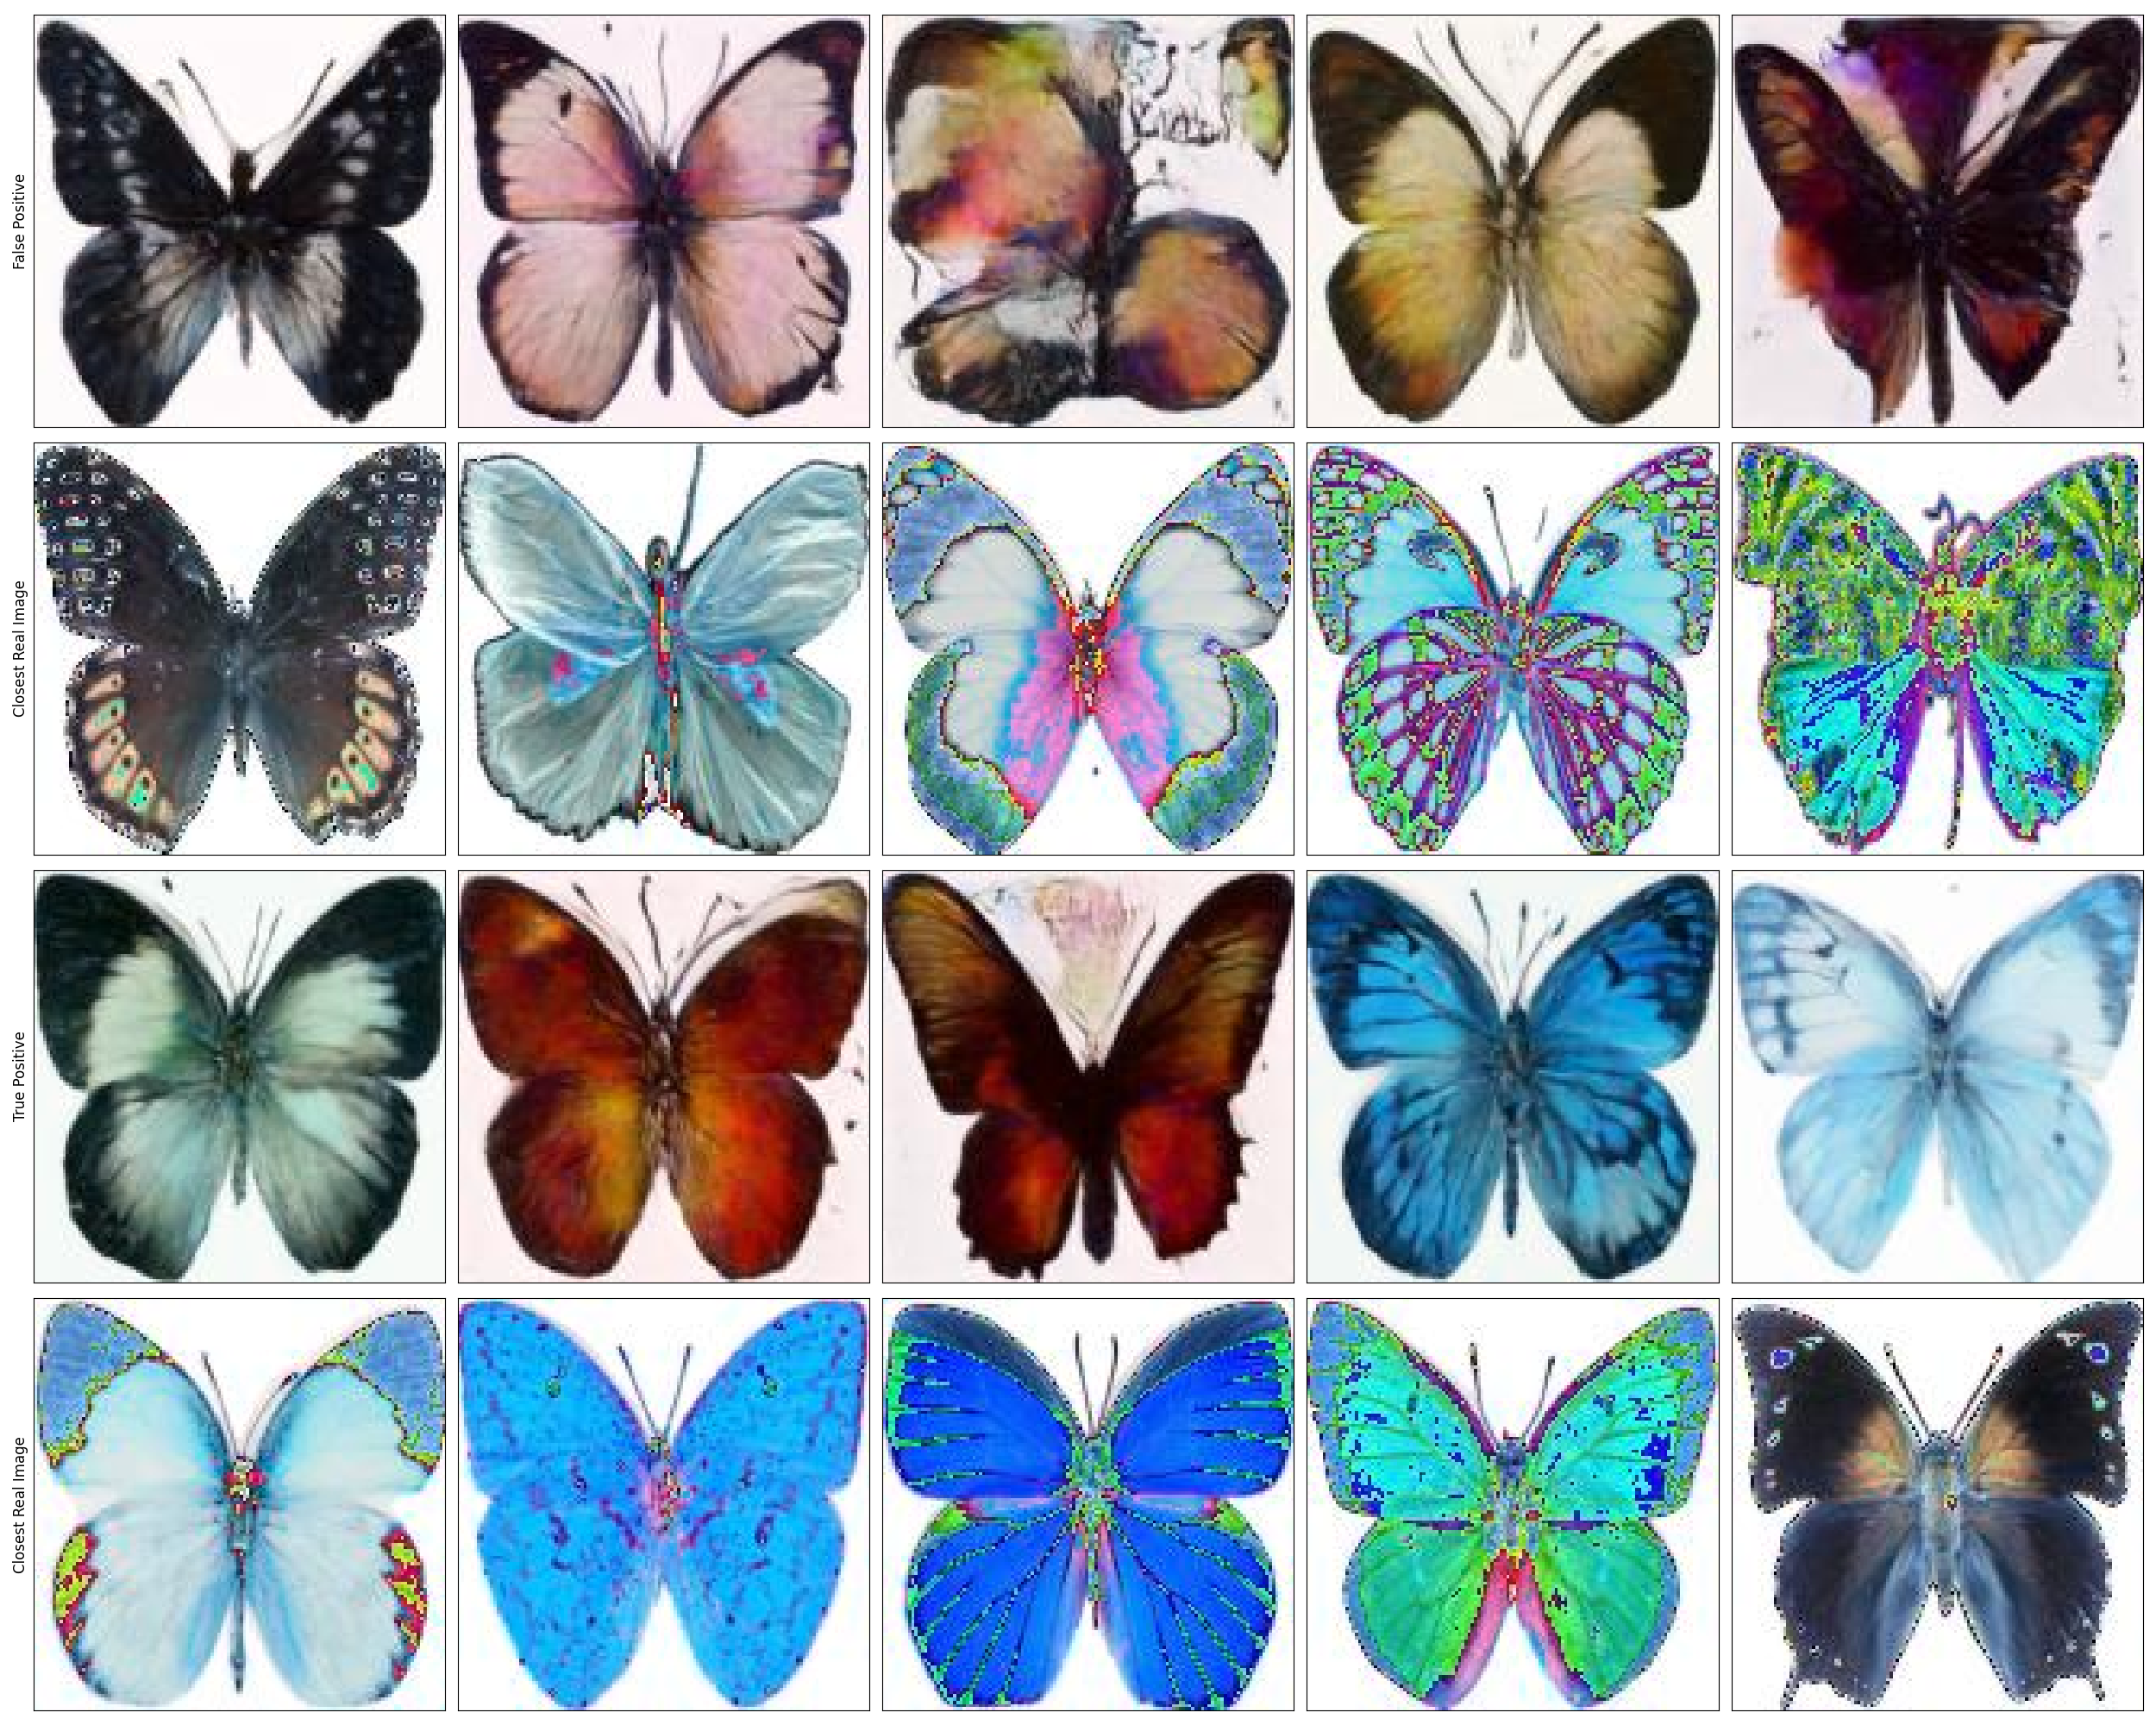
\includegraphics[width=0.45\textwidth]{../images/realworldexperiments/butterflies/examples/fp_saturation_histogram.png}
    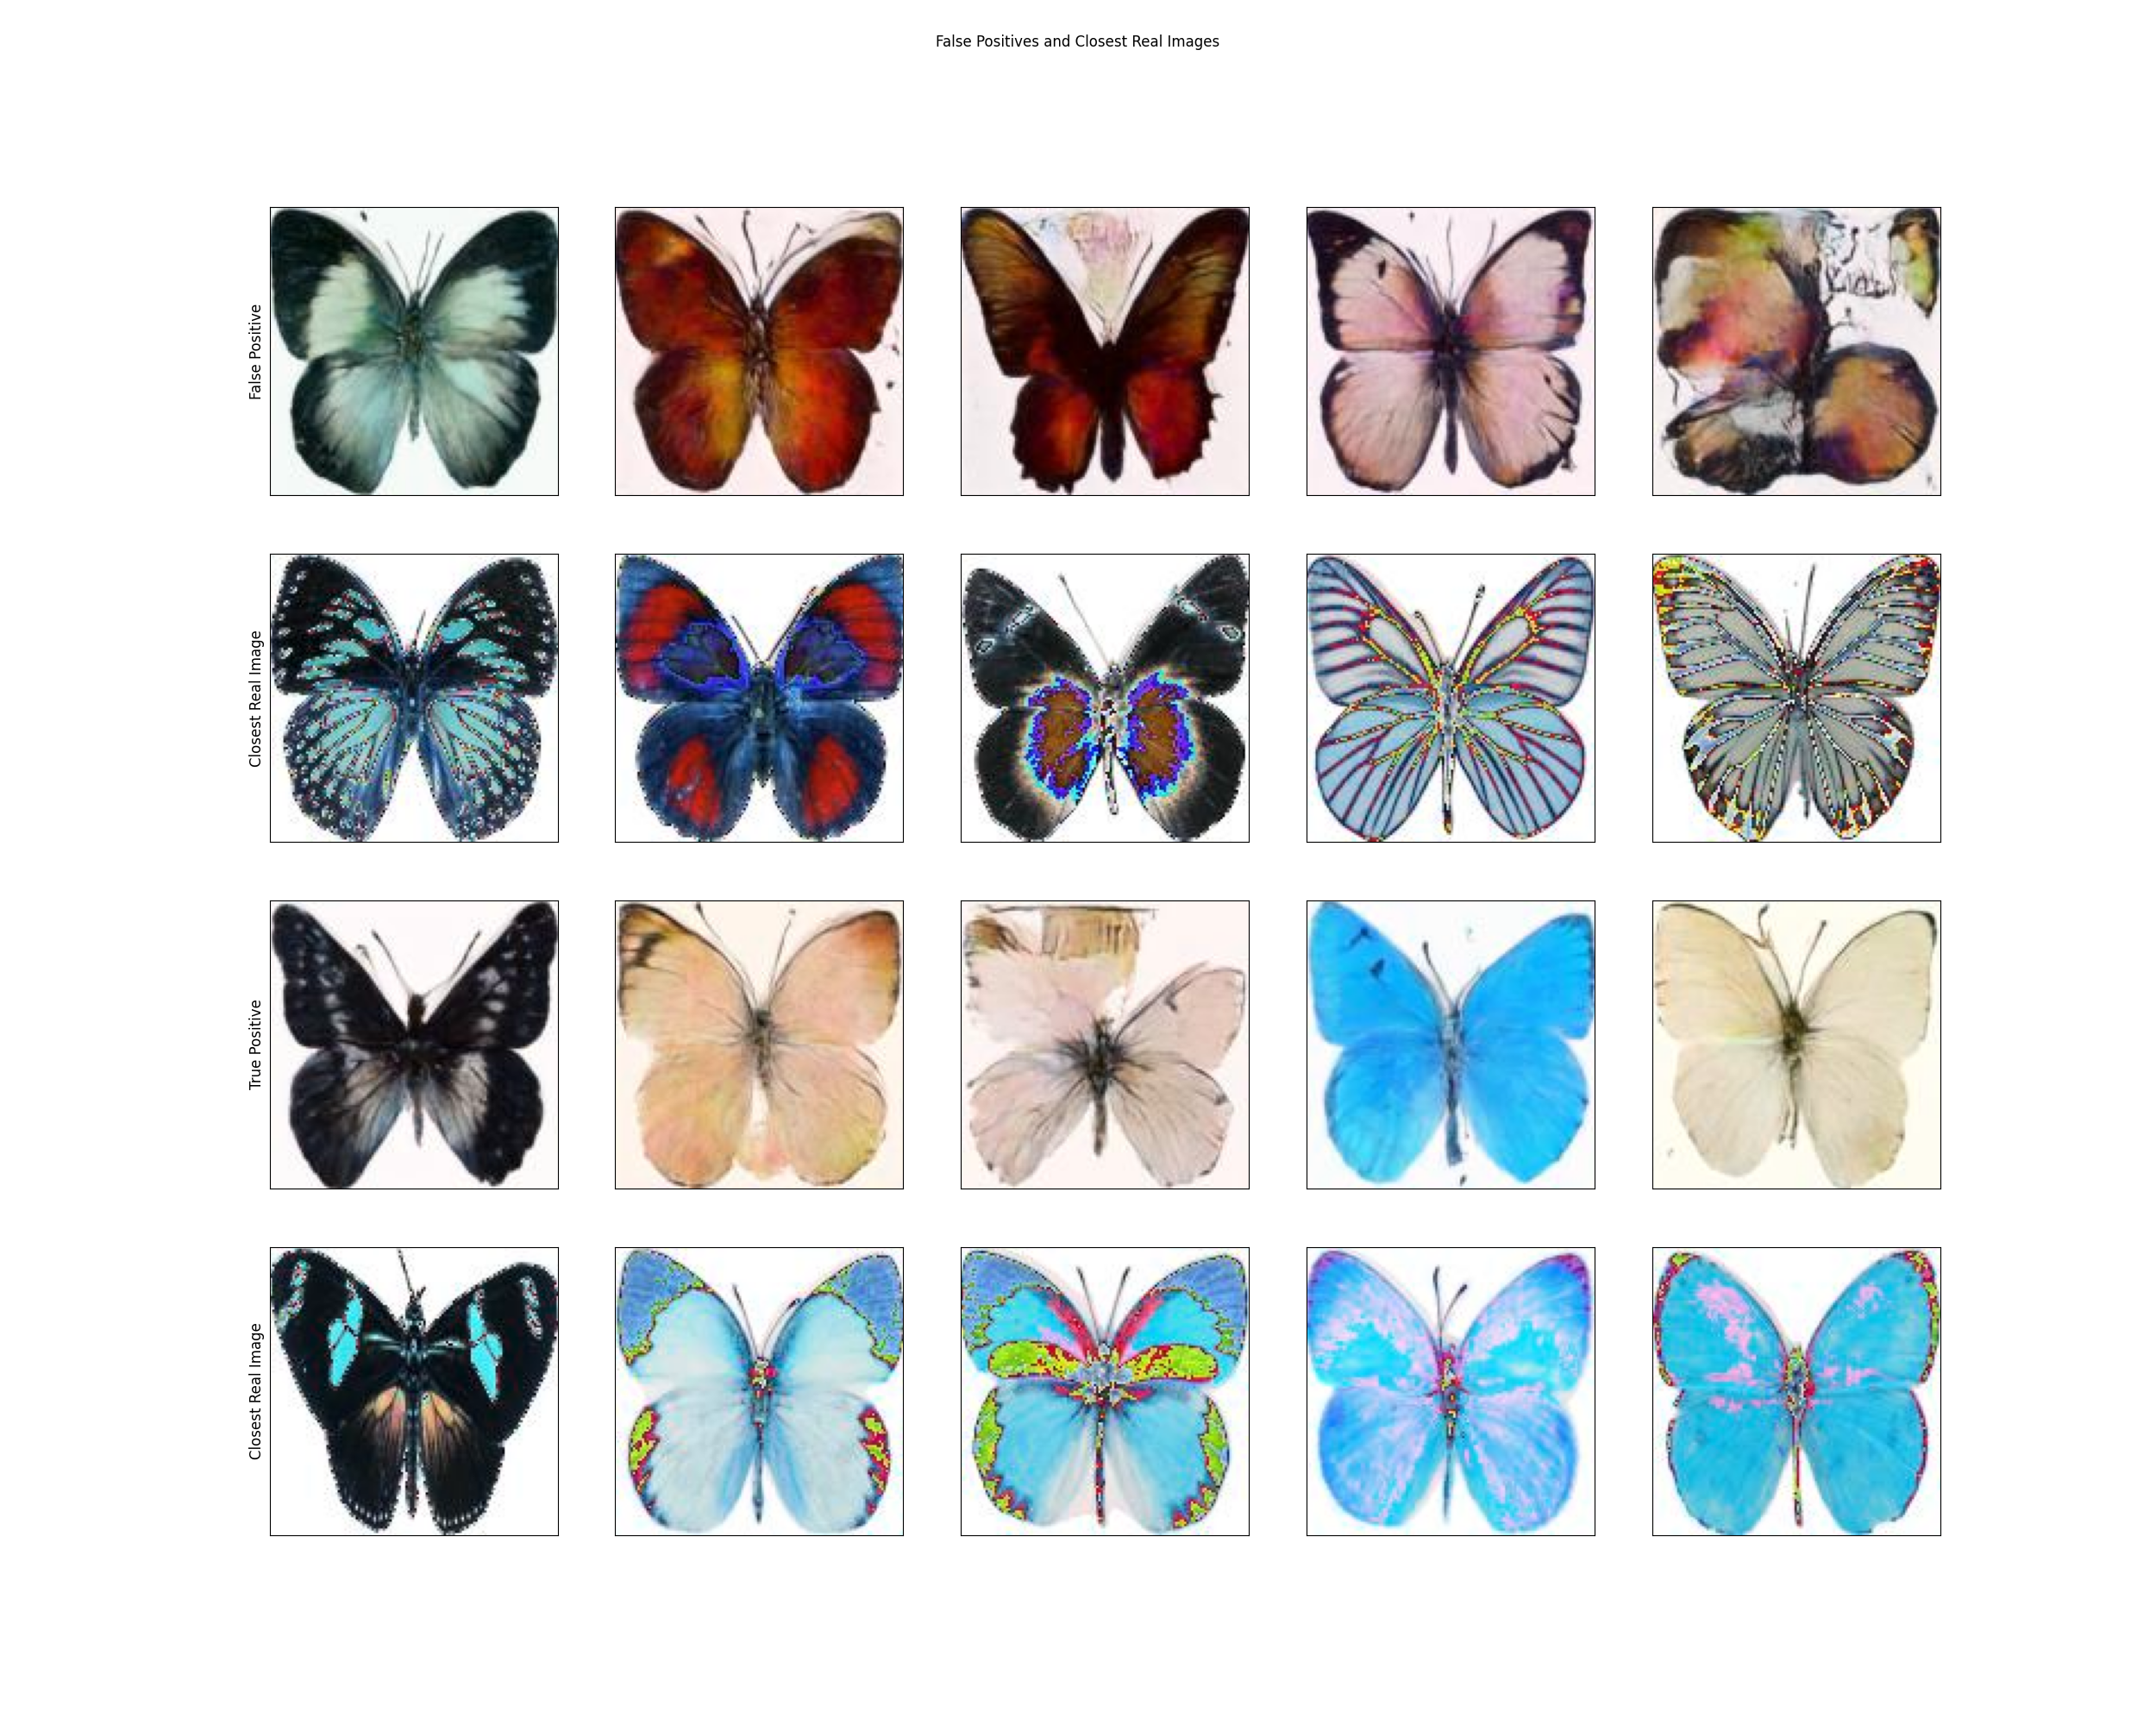
\includegraphics[width=0.45\textwidth]{../images/realworldexperiments/butterflies/examples/fp_value_histogram.png}
    \caption{l'ordine delle immagini da sinistra verso destra e dall'alto in basso è: grayscale, hsv, hue, rgb, saturation, value}
\end{figure}

La maggior parte dei falsi positivi e dei veri positivi sono risultati comuni a tutti gli istogrammi, indicando che questi catturano in modo coerente caratteristiche simili delle immagini.

I falsi positivi presentano frequentemente artefatti visivi o pattern innaturali, mentre i veri positivi, pur essendo più vicini alle immagini reali in termini di colore e luminosità, possono comunque mostrare aberrazioni. Questo è dovuto al fatto che gli istogrammi considerati non catturano informazioni spaziali, ma solo proprietà cromatiche. Le caratteristiche spaziali, fondamentali per identificare la struttura delle immagini, non vengono analizzate in questo approccio, limitando la capacità di distinguere campioni generati di alta qualità.

Ricordiamo inoltre che la selezione si è basata interamente su quei dati che ricadono o meno nel manifold definito dall'improved precision recall, che come visto dagli esperimenti sui toy dataset soffre della presenza di outliers. Dall'analisi della kde risulta che i dati reali sono meno sparsi rispetto ai dati generati, e quindi la presenza di outliers non dovrebbe essere particolarmente influente sull'identificazione dei falsi positivi. Dall'altra parte i dati generati sono più sparsi, è quindi probabile che ci sia una sovrastima del manifold di \(G\), portando a un elevato numero di falsi negativi e veri positivi reali.

I risultati quantitativi delle metriche sono riportati nella Tabella \ref{tab:metriche}. Questi dati evidenziano i compromessi tra precision, recall e altre metriche di performance.

\begin{table}[h!]
    \label{tab:metriche}
    \centering
    \resizebox{\textwidth}{!}{
    \begin{tabular}{lcccccccc}
        \hline
        \textbf{Istogramma} & \textbf{Precision} & \textbf{Recall} & \textbf{Density} & \textbf{Coverage} & \textbf{FPR*} & \textbf{FNR*} & \textbf{n. False Positives} & \textbf{n. True Positives} \\
        \hline
        Hue & 0.4654 & 0.9855 & 0.0720 & 0.1908 & 0.6897 & 0.0402 & 618 & 278 \\
        Saturation & 0.5904 & 0.9978 & 0.1833 & 0.7824 & 0.3996 & 0.0033 & 358 & 538 \\
        HSV & 0.3783 & 0.9866 & 0.0546 & 0.2254 & 0.6719 & 0.0112 & 602 & 294 \\
        RGB & 0.0446 & 0.9978 & 0.0120 & 0.1998 & 0.9096 & 0.0000 & 815 & 81 \\
        Value & 0.2578 & 0.9877 & 0.1113 & 0.7679 & 0.7366 & 0.0022 & 660 & 236 \\
        Grayscale & 0.1071 & 1.0000 & 0.0533 & 0.6763 & 0.9040 & 0.0000 & 810 & 86 \\
        \hline
    \end{tabular}
    }
    \caption{FPR* = False Positive Rate, FNR* = False Negative Rate}
\end{table}

Ai fini di utilizzare la metrica come filtro per i dati generati di alta qualità, siamo poco interessati alla statistica di recall tuttavia è apprezzabile che tutte le distanze considerate abbiano un valore di recall molto alto (che conferma le ipotesi sollevate dall'osservazione della kde).
La precision è molto variabile, con valori che vanno da 0.0446 a 0.5904. Sebbene la saturation registri il valore più alto, come si può vedere dagli esempi visivi, è probabile che la hue sia la metrica più adatta per identificare i falsi positivi.
Questi risultati confermano che, pur fornendo una base solida per l'analisi delle caratteristiche cromatiche, le metriche basate sugli istogrammi richiedono un'integrazione con descrittori spaziali per migliorare la capacità di discriminazione tra dati reali e generati di alta qualità.

\subsection{Scarlatti}

Come descritto nel capitolo precedente \ref{subsec:scarlatti}, i primi esperimenti condotti sul dataset degli Scarlatti sono finalizzati a verificare l'applicabilità della KDE per la rappresentazione delle distribuzione dei dati e a valutare la capacità descrittive delle caratteristiche scelte.
Per fare ciò sono riportati in seguito figura \ref{fig:realworldexperiments-scarlatti-real} i risultati delle KDE applicate alle distanze intra-set per i campioni reali divisi in training set e validation più test set.
Le distribuzioni risultano pressochè identiche, con una leggera differenza dovuta, con molta probabilità, alla diversa dimensione dei due set ( il trainig contiene 920 campioni, il validation 309 e il test 305).

\begin{figure}[!ht]
    \label{fig:realworldexperiments-scarlatti-real}
    \centering
    \includegraphics[width=0.3\textwidth]{../images/realworldexperiments/scarlatti/realdata/TrainVsTest_avgIOI.png}
    \includegraphics[width=0.3\textwidth]{../images/realworldexperiments/scarlatti/realdata/TrainVsTest_avgPitchShift.png}
    \includegraphics[width=0.3\textwidth]{../images/realworldexperiments/scarlatti/realdata/TrainVsTest_nNotesPerMeasure.png}
    \includegraphics[width=0.3\textwidth]{../images/realworldexperiments/scarlatti/realdata/TrainVsTest_noteLengthHist.png}
    \includegraphics[width=0.3\textwidth]{../images/realworldexperiments/scarlatti/realdata/TrainVsTest_noteLengthTransMatrix.png}
    \includegraphics[width=0.3\textwidth]{../images/realworldexperiments/scarlatti/realdata/TrainVsTest_nPitchesPerMeasure.png}
    \includegraphics[width=0.3\textwidth]{../images/realworldexperiments/scarlatti/realdata/TrainVsTest_pitchClassHist.png}
    \includegraphics[width=0.3\textwidth]{../images/realworldexperiments/scarlatti/realdata/TrainVsTest_pitchClassHistPerMeasure.png}
    \includegraphics[width=0.3\textwidth]{../images/realworldexperiments/scarlatti/realdata/TrainVsTest_pitchClassTransMatrix.png}
    \includegraphics[width=0.3\textwidth]{../images/realworldexperiments/scarlatti/realdata/TrainVsTest_pitchRange.png}
    \caption{l'ordine delle immagini da sinistra verso destra e dall'alto in basso è: avgIOI, avgPitchShift, nNotesPerMeasure, noteLengthHist, noteLengthTransMatrix, nPitchesPerMeasure, pitchClassHist, pitchClassHistPerMeasure, pitchClassTransMatrix, pitchRange}
\end{figure}

Possiamo notare che una delle caratteristiche, la \textbf{pitchRange}, presenta una distribuzione che, sebbene sia molto simile per i due set, fallisce l'approssimazione della bandwidth della KDE, portando alla presenza di picchi multipli. Questo è dovuto, oltre che alla scalarità della feature, alla sua discretezza.
I pitch range potendo assumere solo valori interi presenterà delle distanze intra-set intere a loro volta, e quindi la KDE non sarà in grado di approssimare correttamente la distribuzione. Gli esperimenti successivi riporteranno comunque i risultati per questa feature, ma è fondamentale ridimensionarne l'importanza.

Si passa ora alla valutazione delle metriche per i dati generati. I risultati ottenuti sono riportati in figura \ref{fig:realworldexperiments-scarlatti-fake}.

\begin{figure}[!ht]
    \centering
    \includegraphics[width=0.6\textwidth]{../images/realworldexperiments/scarlatti/violinplots/TrainVsFake_avgIOI.png}
    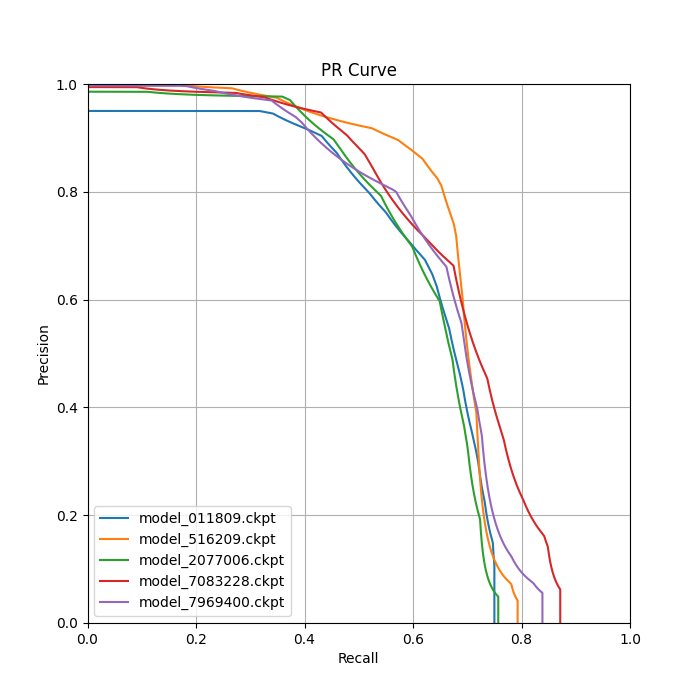
\includegraphics[width=0.3\textwidth]{../images/realworldexperiments/scarlatti/prcurves/PRCurveScarlatti_avgIOI.png}
\end{figure}
\begin{figure}[!ht]
    \centering
    \includegraphics[width=0.6\textwidth]{../images/realworldexperiments/scarlatti/violinplots/TrainVsFake_avgPitchShift.png}
    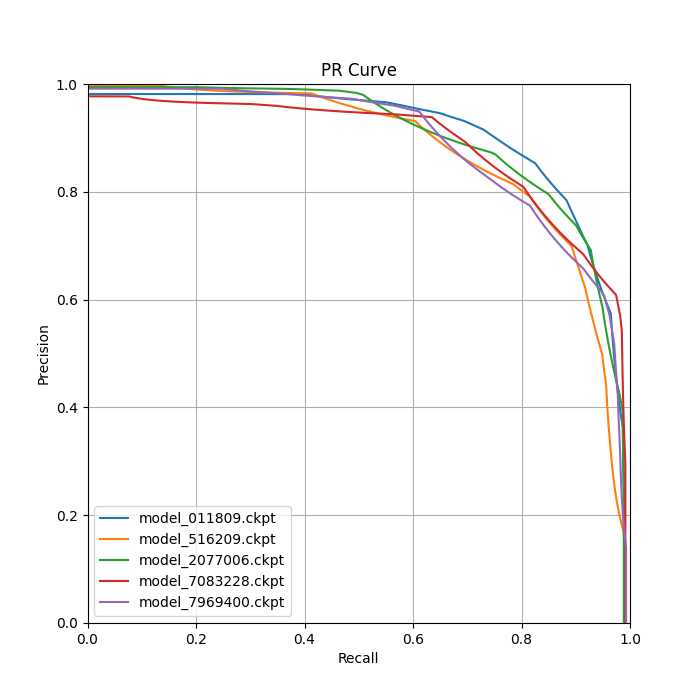
\includegraphics[width=0.3\textwidth]{../images/realworldexperiments/scarlatti/prcurves/PRCurveScarlatti_avgPitchShift.png}
\end{figure}  
\begin{figure}[!ht]
    \centering
    \includegraphics[width=0.6\textwidth]{../images/realworldexperiments/scarlatti/violinplots/TrainVsFake_nNotesPerMeasure.png}
    \includegraphics[width=0.3\textwidth]{../images/realworldexperiments/scarlatti/prcurves/PRCurveScarlatti_nNotesPerMeasure.png}
\end{figure} 
\begin{figure}[!ht]
    \centering
    \includegraphics[width=0.6\textwidth]{../images/realworldexperiments/scarlatti/violinplots/TrainVsFake_noteLengthHist.png}
    \includegraphics[width=0.3\textwidth]{../images/realworldexperiments/scarlatti/prcurves/PRCurveScarlatti_noteLengthHist.png}
\end{figure}   
\begin{figure}[!ht]
    \centering
    \includegraphics[width=0.6\textwidth]{../images/realworldexperiments/scarlatti/violinplots/TrainVsFake_noteLengthTransMatrix.png}
    \includegraphics[width=0.3\textwidth]{../images/realworldexperiments/scarlatti/prcurves/PRCurveScarlatti_noteLengthTransMatrix.png}
\end{figure}   
\begin{figure}[!ht]
    \centering
    \includegraphics[width=0.6\textwidth]{../images/realworldexperiments/scarlatti/violinplots/TrainVsFake_nPitchesPerMeasure.png}
    \includegraphics[width=0.3\textwidth]{../images/realworldexperiments/scarlatti/prcurves/PRCurveScarlatti_nPitchesPerMeasure.png}
\end{figure}  
\begin{figure}[!ht]
    \centering
    \includegraphics[width=0.6\textwidth]{../images/realworldexperiments/scarlatti/violinplots/TrainVsFake_pitchClassHist.png}
    \includegraphics[width=0.3\textwidth]{../images/realworldexperiments/scarlatti/prcurves/PRCurveScarlatti_pitchClassHist.png}
\end{figure}
\begin{figure}[!ht]
    \centering
    \includegraphics[width=0.6\textwidth]{../images/realworldexperiments/scarlatti/violinplots/TrainVsFake_pitchClassHistPerMeasure.png}
    \includegraphics[width=0.3\textwidth]{../images/realworldexperiments/scarlatti/prcurves/PRCurveScarlatti_pitchClassHistPerMeasure.png}
\end{figure}
\begin{figure}[!ht]
    \centering
    \includegraphics[width=0.6\textwidth]{../images/realworldexperiments/scarlatti/violinplots/TrainVsFake_pitchClassTransMatrix.png}
    \includegraphics[width=0.3\textwidth]{../images/realworldexperiments/scarlatti/prcurves/PRCurveScarlatti_pitchClassTransMatrix.png}
\end{figure}
\begin{figure}[!ht]
    \label{fig:realworldexperiments-scarlatti-fake}
    \centering
    \includegraphics[width=0.6\textwidth]{../images/realworldexperiments/scarlatti/violinplots/TrainVsFake_pitchRange.png}
    \includegraphics[width=0.3\textwidth]{../images/realworldexperiments/scarlatti/prcurves/PRCurveScarlatti_pitchRange.png}
    \caption{l'ordine delle immagini dall'alto in basso è: avgIOI, avgPitchShift, nNotesPerMeasure, noteLengthHist, noteLengthTransMatrix, nPitchesPerMeasure, pitchClassHist, pitchClassHistPerMeasure, pitchClassTransMatrix, pitchRange}
\end{figure}

Si può notare una generale tendenza delle pr-curves a confermare quanto osservato anche nelle kde. Come sollevato in ipotesi, per molte delle metriche si nota che con il passare delle epoche il modello generativo tende a generare dati sempre più simili a quelli reali, e quindi la sovrapposizione dei manifold di \(G\) e \(R\) aumenta.
In particolare il fenomeno è più evidente per le distanze matriciali quali \textbf{noteLengthTransMatrix} e \textbf{pitchClassTransMatrix}, e per il numero di altezze diverse per misura \textbf{nPitchesPerMeasure}. Meno marcato invece per le distanze scalari.
Un altro aspetto interessante è che, a meno delle \textbf{pitchClassHist} e \textbf{pitchClassTransMatrix} il modello generativo produce buoni risultati già alla seconda epoca di allenamento considerata, che risulta la migliore per numero di note per misura e per l'istogramma delle lunghezza delle note.
Questi risultati che vediamo nei grafici sono verificati anche numericamente, vedi tabella \ref{tab:res-scarlatti-supp}.

\begin{table}[h!]
    \textbf{Model - 011809}
    \centering
    \resizebox{\textwidth}{!}{
    \begin{tabular}{lccccccc}
        \hline
        \textbf{Feature} & \textbf{IP} & \textbf{IR} & \textbf{Density} & \textbf{Coverage} & \textbf{FPR} & \textbf{FNR} & \textbf{OA}\\ 
        \hline
        nNotesPM&0.6044&0.8956&0.3674&0.3911&0.3333&0.0822&0.7442 \\
        nPitchesPM&0.7211&0.9100&0.4904&0.5556&0.1922&0.0578&0.8335 \\
        pitchHist&0.8522&0.7978&0.7881&0.6611&0.2156&0.1811&0.7608 \\
        pitchHistPM&0.5489&0.6200&0.4296&0.5167&0.3811&0.3044&0.8639 \\
        pitchTrans&0.7311&0.2156&0.9330&0.5589&0.3578&0.6878&0.6215 \\
        pitchRange&0.0744&0.0267&0.0626&0.0122&0.0244&0.0144&0.9506 \\
        avgPitchShift&0.9189&0.9300&0.8807&0.7967&0.0189&0.0333&0.9477 \\
        avgIOI&0.4889&0.4322&0.3626&0.2833&0.1478&0.1000&\cellcolor{green}0.9178 \\
        lengthHist&0.7711&0.8800&0.7874&0.7522&0.2322&0.1056&0.8427 \\
        lengthHistPM&0.7811&0.8611&0.7511&0.7067&0.2411&0.1511&0.8656 \\
        lengthTrans&0.9489&0.7933&1.0593&0.6433&0.1656&0.2400&0.9043 \\
        \hline
    \end{tabular}
    }
\end{table}
\begin{table}[h!]
    \textbf{Model - 516209}
    \centering
    \label{tab:res-scarlatti-supp}
    \resizebox{\textwidth}{!}{
    \begin{tabular}{lccccccc}
        \hline
        \textbf{Feature} & \textbf{IP} & \textbf{IR} & \textbf{Density} & \textbf{Coverage} & \textbf{FPR} & \textbf{FNR} & \textbf{OA} \\ 
        \hline
        nNotesPM&0.7933&0.7900&0.6074&0.6278&\cellcolor{green}0.1533&0.1656&\cellcolor{green}0.8671 \\
        nPitchesPM&0.7978&0.7789&0.6793&0.6833&0.1178&0.1522&0.8758 \\
        pitchHist&0.9078&0.8511&1.0900&0.7956&0.0833&0.1800&0.9018 \\
        pitchHistPM&0.6222&0.6578&0.5841&0.6900&0.2733&0.2544&0.9118 \\
        pitchTrans&0.8978&0.3533&1.8900&0.8711&0.0911&0.6167&0.7370 \\
        pitchRange&0.0311&0.0222&0.0300&0.0144&0.0044&0.0122&\cellcolor{green}0.9809 \\
        avgPitchShift&0.9233&0.9067&0.8752&0.7867&0.0200&0.0489&0.9688 \\
        avgIOI&0.3778&0.3222&0.3078&0.2589&\cellcolor{green}0.0700&0.0933&0.8926 \\
        lengthHist&0.8600&0.8356&0.9978&0.8167&\cellcolor{green}0.1611&0.1656&\cellcolor{green}0.9335 \\
        lengthHistPM&0.8256&0.7967&0.8678&0.7778&\cellcolor{green}0.1122&0.2189&0.9497 \\
        lengthTrans&0.9722&0.8144&1.1374&0.7789&\cellcolor{green}0.0556&0.2500&0.9002 \\
        \hline
    \end{tabular}
    }
\end{table}
\begin{table}[h!]
    \textbf{Model - 2077006}
    \centering
    \resizebox{\textwidth}{!}{
    \begin{tabular}{lccccccc}
        \hline
        \textbf{Feature} & \textbf{IP} & \textbf{IR} & \textbf{Density} & \textbf{Coverage} & \textbf{FPR} & \textbf{FNR} & \textbf{OA} \\ 
        \hline
        nNotesPM&0.7533&0.8611&0.5519&0.5944&0.1878&0.1067&0.8549 \\
        nPitchesPM&0.7778&0.8300&0.6130&0.6467&0.1378&0.1311&0.9122 \\
        pitchHist&0.9111&0.8911&0.9100&0.8356&0.0856&0.0933&0.9111 \\
        pitchHistPM&0.6289&0.7733&0.5578&0.6622&0.2356&0.1589&0.9347 \\
        pitchTrans&0.8911&0.5789&1.2419&0.8778&0.1056&0.3711&0.9266 \\
        pitchRange&0.0289&0.0056&0.0241&0.0133&0.0022&0.0033&0.9283 \\
        avgPitchShift&0.9100&0.9222&0.8656&0.7844&0.0244&0.0422&0.9744 \\
        avgIOI&0.4467&0.4222&0.3533&0.2711&0.1278&0.0556&0.8827 \\
        lengthHist&0.7856&0.8933&0.7659&0.7478&0.2200&0.1100&0.8624 \\
        lengthHistPM&0.8156&0.8689&0.8567&0.7767&0.1611&0.1611&\cellcolor{green}0.9765 \\
        lengthTrans&0.9367&0.8811&1.0404&0.8333&0.1011&0.1733&0.9595 \\
        \hline
    \end{tabular}
    }
\end{table}
\begin{table}[h!]
    \textbf{Model - 7083228}
    \centering
    \resizebox{\textwidth}{!}{
    \begin{tabular}{lccccccc}
        \hline
        \textbf{Feature} & \textbf{IP} & \textbf{IR} & \textbf{Density} & \textbf{Coverage} & \textbf{FPR} & \textbf{FNR} & \textbf{OA} \\ 
        \hline
        nNotesPM&0.7767&0.8456&0.5937&0.6167&0.1767&0.1211&0.8615 \\
        nPitchesPM&0.8156&0.8333&0.6463&0.6867&\cellcolor{green}0.1067&0.1033&\cellcolor{green}0.9518 \\
        pitchHist&0.9200&0.9111&0.9515&0.8689&0.0789&0.1056&0.9458 \\
        pitchHistPM&0.7322&0.7722&0.6519&0.7556&0.1656&0.1744&0.9305 \\
        pitchTrans&0.8911&0.7122&1.1104&0.9089&\cellcolor{green}0.0856&0.2589&\cellcolor{green}0.9719 \\
        pitchRange&0.0478&0.0056&0.0426&0.0167&\cellcolor{green}0.0000&0.0022&0.9704 \\
        avgPitchShift&0.9156&0.9000&0.8641&0.8067&0.0267&0.0356&0.9474 \\
        avgIOI&0.4633&0.4656&0.3493&0.2622&0.1344&0.0589&0.9006 \\
        lengthHist&0.7978&0.9100&0.7593&0.8067&0.1778&0.0978&0.8585 \\
        lengthHistPM&0.8378&0.8811&0.8859&0.8233&0.1344&0.1322&0.9657 \\
        lengthTrans&0.9267&0.8978&0.9889&0.8311&0.1111&0.1244&0.9693 \\
        \hline
    \end{tabular}
    }
\end{table}
\begin{table}[h!]
    \textbf{Model - 7969400}
    \centering
    \resizebox{\textwidth}{!}{
    \begin{tabular}{lccccccc}
        \hline
        \textbf{Feature} & \textbf{IP} & \textbf{IR} & \textbf{Density} & \textbf{Coverage} & \textbf{FPR} & \textbf{FNR} & \textbf{OA} \\ 
        \hline
        nNotesPM&0.7922&0.8289&0.6074&0.6167&0.1567&0.1289&0.8574 \\
        nPitchesPM&0.8156&0.8578&0.6822&0.7367&0.1133&0.0922&0.9425 \\
        pitchHist&0.9256&0.8967&0.9215&0.8667&\cellcolor{green}0.0722&0.1167&\cellcolor{green}0.9548 \\
        pitchHistPM&0.7456&0.7656&0.6800&0.7767&\cellcolor{green}0.1489&0.1767&\cellcolor{green}0.9491 \\
        pitchTrans&0.8922&0.7000&1.0985&0.9011&0.1133&0.2567&0.9700 \\
        pitchRange&0.0389&0.0056&0.0348&0.0167&0.0033&0.0000&0.9504 \\
        avgPitchShift&0.9322&0.9256&0.8930&0.8144&\cellcolor{green}0.0156&0.0400&\cellcolor{green}0.9897 \\
        avgIOI&0.4367&0.4322&0.3478&0.2656&0.1144&0.0478&0.8864 \\
        lengthHist&0.8111&0.8933&0.7648&0.7744&0.1789&0.1033&0.8685 \\
        lengthHistPM&0.8489&0.8644&0.8870&0.8178&0.1144&0.1589&0.9499 \\
        lengthTrans&0.9378&0.8956&1.0115&0.8656&0.1033&0.1433&\cellcolor{green}0.9614 \\
        \hline
    \end{tabular}
    }
    \caption{I risultati ottenuti con l'identificazione dei falsi positivi tramite supporto (indicata con OA l'Overlapped Area)}
\end{table}

Quello che si nota e che giustifica gli esperimenti successivi è che non sempre c'è una corrispondenza fra il modello con minor numero di falsi positivi e maggior overlapped area. Questo vale in particolare proprio per il modello appena citato, il 516209, che presenta spesso il maggior numero di falsi positivi ma anche il maggior numero di falsi negativi. 
Se si osserva i valori della density e della coverage possiamo facilmente stabilire che questa epoca tende a generare dati con poca varianza, \textit{diversity}. Vogliamo quindi verificare se si ottengono gli stessi risultati operando invece che con il supporto dell'improved precision-recall, con le kde.
Utilizzare un diverso approccio permette, oltre che mezzo di confronto, controprova per la validità dei risultati ottenuti. 

Come indicato nel capitolo precedente \ref{subsec:scarlatti}, utilizzando un percentile fisso per la selezione dei falsi positivi, si ottiene sempre lo stesso numero di outliers indipendentemente dal modello. Tuttavia si può verificare sperimentalmente che i risultati prodotti sono migliori rispetto a quelli ottenuti con il supporto dell'improved precision-recall. 
Un ascolto degli esempi raccolti con questo metodo verifica immediatamente che i falsi positivi sono effettivamente dati generati di bassa qualità, sono infatti discriminati quei dati mal generati che non hanno il numero corretto di misure, sono individuati i dati che tendono a ripetere sempre la stessa nota e lo stesso vale per i dati che presentano pause o passaggi armonici poco naturali.
